\chapter{Joint ISR-Optical Tomography Analysis}
\label{chapter:fusion}
\thispagestyle{myheadings}

\graphicspath{{Fusion/}}

\epigraph{In order to solve the problem of the cause of the aurora and magnetic perturbations, it was necessary to have at our command simultaneous magnetograms and observations from several suitable polar stations at distances of about 1000 kilometers from one another, and also corresponding material from as many other stations all over the world as it was possible to obtain. I demonstrated namely, that certain well-defined magnetic perturbations that occurred over large portions of the earth might be naturally explained as the effect of electric currents.}{\citep{birkeland1908}}

Alfvén waves are an important mechanism for communicating magnetospheric stress into Earth's upper atmosphere.
A significant fraction of the Alfvénic flux is realized as ionospheric Langmuir turbulence and thin dynamic auroral arcs.
Key signatures of Alfvénic dispersion are revealed in the spatiotemporal structure of the aurora. 
Alfvénic auroral structures are strikingly distinct from auroral arcs produced by quasi-static parallel electric fields.
Distinguishing quasi-static arcs from Alfvénic arcs requires high-speed, high-resolution filtered optical systems to capture prompt emissions.
Coordinated optical and incoherent scatter radar measurements routinely show strong echoes from ionospheric destabilization spatiotemporally associated with Alfvénic aurora.
Such observations suggest a connection between Alfvénic particle flux and destabilization of ion-acoustic and Langmuir (electron-acoustic) waves in the lower ionosphere.
The utility of a ground-based high-speed optical tomography system providing estimates of electron precipitation energy spectral characteristics during Alfvén-wave driven destabilization is demonstrated.

\graphicspath{{Fusion/}}

\section{Introduction}\label{sec:intro}
Thin beams of intense electron precipitation are associated with spatially discrete aurora and families of wave modes arising from the beam-destabilized plasma \citep{akbari2015}.
Incoherent scatter radar (ISR) routinely shows F-region enhancements in the ion-acoustic and plasma line spectra associated with wave mode destabilization due to this intense precipitation \citep{schlatter2014}.
Optical measurements of finely structured prompt auroral emissions are strongly correlated with incoherent scatter radar (ISR) backscatter power \citep{sullivan2008,michell2009,michell2014}.
Fast-sampling auroral tomography systems can estimate particle precipitation differential number flux as a function of space, energy and time based on prompt auroral emissions \citep{hirsch2016}.
It is often difficult to determine the direct mechanism by which the energy of the precipitating particles is transformed into free energy for plasma waves.
The exact mechanism underlying the intensification of ion-acoustic waves regularly observed by ISRs in the form of strong backscattered echoes called NEIALs (Naturally Enhanced Ion Acoustic Lines) is not well understood \citep{michell2014}.
In the case of NEIALs there exist competing theories that relate the free energy to fluxes of soft electron precipitation \citep{akbari2014} or to populations of thermal electrons and ions streaming relative to one another \citep{akbari2012}.

Guided by prior observational and theoretical knowledge of spatiotemporal bounds on ground-observable physics, researchers over the past century \citep{stormer1930,stormer1932} and especially the past decade \citep{lynch2012,donovan2006,dahlgren2008} have infused technological progress into systems designed for better understanding of magnetospheric particle precipitation via optical measurements of aurora.
\citet{semeter2008} used a single \unit[30]{fps} $512 \times 512$ pixel BG3-filtered EMCCD camera with PFISR to study dispersive Alfvén wave (DAW) aurora during an substorm breakup, where thin filaments periodically and rapidly split from the arc. 
The splitting arc optical signature is a manifestation of the dispersion relation of DAW with a spatially periodic structure \citep{semeter2008}.
\citet{dahlgren2013} used bursts of a single \unit[30]{fps} sCMOS $2560 \times 2160$ pixel BG3-filtered camera with Poker Flat ISR (PFISR) to characterize flaming aurora with sub-second time scales.
Flaming aurora \citep{omholtbook,dahlgren2013} is generated by DAW auroral flux with faster high energy particles arriving first in the lower ionosphere.
The MOOSE instrument \citep{michell2014} consists of four co-aimed $190 \times 190$ pixel EMCCD cameras running at 40 frames/s with filters for $\lambda \in \{427.8, 844.6, 630.0\}$~nm and a BG3 filter.
The High Speed Auroral Tomography system (HiST) \citep{hirsch2016} yields estimates of primary precipitating electron differential number flux at \unit[20]{ms} cadence.
Faster frame rates are constrained by the SNR achievable from -60$^\circ$C cooled EMCCD cameras sensitive to single photoelectrons, considering the optical filtering needed to select prompt emissions.

Characterizing various types of tightly $B_\perp$-spaced DAW auroral arcs requires networks of cameras spaced in the \unit[1..10]{km} range as simulated in Figure~\ref{fig:camres}.
The HiST synchronized cameras enable detection of conditions favorable for plasma turbulence from auroral arcs.
Examples of discrete auroral arcs are drawn in Figure~\ref{fig:cartoonmorph}.
\begin{figure}\centering
	\begin{minipage}{0.3\textwidth}\centering
		\includegraphics[width=0.9\columnwidth,trim=150 100 150 100,clip]{gfx/aurora_kinked}
	\end{minipage}
	\begin{minipage}{0.3\textwidth}\centering
		\includegraphics[width=0.9\columnwidth,trim=150 100 150 100,clip]{gfx/aurora_split}
	\end{minipage}
	\begin{minipage}{0.3\textwidth}\centering
		\includegraphics[width=0.9\columnwidth,trim=150 100 150 100,clip]{gfx/aurora_ray}
	\end{minipage}
	\caption{Auroral arc morphologies corresponding to: 
		(a) inverted-V 
		(b) strong Langmuir turbulence 
		(c) streaming upflow}
	\label{fig:cartoonmorph}
\end{figure}
This article presents the first joint analysis of such high-speed, closely spaced multi-camera auroral video using physics model-based iterative reconstruction.
The system is shown to be capable of distinguishing monoenergetic inverted-V electron precipitations (with characteristic energy of several keV) from broadband (tens of eV to several keV) electron precipitations from DAW.
New radar sampling techniques \citep{swoboda2015} enable increasingly fine spatio-temporal resolution suitable for quantifying NEIAL characteristics \citep{schlatter2015}.
ISR measurement cadence of \unit[12]{ms} for ion-line \citep{michell2010} and \unit[200]{ms} for plasma-line \citep{vierinen2016} have been achieved, a factor of 80 improvement over prior plasma-line measurements \citep{nicolls2006}.
Joint optical and ISR measurements targeting NEIALs need to sample faster than \unit[40]{Hz} to capture the temporal dynamics of NEIALs.
Persistent staring automated instruments are required for a practical systems since an entire NEIAL event may last less than half a second \citep{dahlgren2013}.

Joint ISR and high speed filtered optical observations give supporting evidence for apparent connections between DAW aurora and naturally enhanced ion-acoustic lines (NEIALs).
NEIALs are bursty aspect-angle dependent strong ion-line echoes in the lower ionosphere.
Strong echoes in the plasma-line channel accompanied by NEIALs are from Langmuir waves, associated with large fluxes of precipitating electrons \citep{akbari2012}.
The primary electron differential number flux associated with NEIALs has similar sub-second temporal scales and $B_\perp$ scale of \unit[100]{m}.
$B_\perp$ scale width due to anthropogenic heating such as HAARP leads to \unit[100]{m} $B_\perp$ auroral emissions \citep{kelley1995,kendall2010}.
During NEIALs, the ISR fitter algorithms relying upon a Maxwellian ion distribution break down due to non-Maxwellian ion spectrum \citep{knudsen1993}, leading to derived plasma parameters in large error or NaN values.
The mechanisms driving NEIALs are distinct from the electron convection responsible for strong backscatter from Farley-Buneman instabilities arising in the E-region ionosphere below \unit[130]{km} \citep{oppenheim1996,hysell2013}.
Simulation efforts to characterize NEIALs are underway \citep{diaz2008}, but push modern supercomputers such as STAMPEDE to the limits.

\citet{akbari2012} noted open questions on the specific energy transport and deposition processes generating the ionospheric plasma destabilization.
Two possibilities for the energy deposition generating the turbulence are:
\begin{enumerate}
    \item plasma waves intensified directly by primary electron precipitation kinetic processes
    \item plasma waves intensified by secondary suprathermal (hundreds of eV) electrons as a result of the electron beam.
\end{enumerate}
Particle acceleration yielding narrow $B_\perp$ energy flux structure from the magnetosphere into the ionosphere may come from quasi-static electric fields or Alfvén waves.
\citet{akbari2014} speculated that diverse electron precipitation mechanisms may be responsible for driving NEIALs, due to the strong aspect angle dependence of ISR returns.
Rocket observations \citep{knudsen1990} have provided \textit{in situ} measurements distinguishing Alfvén wave accelerated particles from quasi-static accelerated particles.
Since NEIALs may occur for only a few seconds during a substorm, confirmation via \textit{in situ} measurement would take numerous million-dollar rocket launches, each yielding a few minutes of data.
Practical observational means associating Alfvén waves with the turbulence arises from ground-based high speed synchronized cameras used together with ISR.
\graphicspath{{Fusion/}}
%\citet{akbari2012} discussed Langmuir turbulence using low-level radar data using a single high-speed EMCCD camera.
%\citet{dahlgren2013} gave relative estimates of flaming auroral behavior with an EMCCD camera and PFISR-based starting assumptions.
Fast EMCCD camera observations with ISR routinely show thin, highly dynamic aurora with temporal signatures characteristic of DAW aurora.
Shear plasma flows such as occur during reconnection launch Alfvén waves of wavenumber short enough to be seen in $\sim$ 10 degree field of view (FOV) cameras focused on a region about magnetic zenith.
During active solar times, substorms occur frequently enough that multiple Alfvénic aurora may be observed in a single night.
The following subsections describe the instruments and methods used to distinguish inverted-V aurora from the Alfvénic aurora associated with NEIALs.

\FloatBarrier
\subsection{Poker Flat ISR (PFISR)}\label{sec:fuspfisr}
PFISR produces several low-level data products including the complex analog-to-digital converter voltage samples.
At the time, access to the large files containing low-level PFISR data is by request, with radar data accumulating at $\sim \unit[1.5]{MB/s}$ during a typical experiment.
% data: Apr 14 2013  (468530486 + 224263860 + 224263860 + 187839490) bytes / 729 seconds = 1.516 MByte/sec
Madrigal PFISR high-level data products have integration times $\sim \unit[2]{min}$ versus \unit[10..100]{ms} cadence of the low-level PFISR data.
Long integration time is necessary for plasma parameter estimation since incoherent returns from the ionospheric volume target provide return signals far too weak to characterize from a single pulse.
An autocorrelation function (ACF) is built up from the incoherent electron and ion scatterers over tens of seconds.
Taking the Fourier transform of the ACF the power spectral density (PSD) is obtained, with a notional PSD from a quiet ionosphere shown in Figure~\ref{fig:isrmorph}(a).
An ACF fitting algorithm provides estimates of electron number density, electron and ion temperature and ion velocity.

These plasma parameter estimates break down when turbulent plasma leads to a breakdown in the parameter fitter, which expects PSDs having morphology similar to Figure~\ref{fig:isrmorph}(a).
Strong Langmuir turbulence \citep{akbari2012} leads to ISR spectrum like that depicted in Figure~\ref{fig:isrmorph}(b).
\begin{figure}\centering
    \includegraphics[width=0.8\columnwidth,trim=80 260 100 280,clip]{gfx/isr_thermal}

    \includegraphics[width=0.8\columnwidth,trim=80 260 100 270,clip]{gfx/isr_slt}

    \includegraphics[width=0.8\columnwidth,trim=80 260 100 270,clip]{gfx/isr_streamupflow}
    \caption{(a) Notional PFISR spectrum for quiet ionospheric conditions. 
    	(b) Notional PFISR spectrum under strong Langmuir turbulence. 
    	(c) Notional PFISR spectrum with streaming upflowing plasma.}
    \label{fig:isrmorph}
\end{figure}
Streaming upflows lead to ISR spectrum similar to the depiction in Figure~\ref{fig:isrmorph}(c).
The ISR fitter algorithm used in plasma parameter estimation assumes a single-Maxwellian distribution, which breaks down under turbulent conditions, leading to non-physical plasma parameter estimates.
Alfvénic aurora associated with this Langmuir turbulence leaves fingerprints in the auroral morphology HiST was designed to observe.

The PFISR complex vector $\mathbf{I}+j\mathbf{Q}$ sampled time series is obtained with revisit time as fast as \unit[75]{ms} \citep{akbari2012} for five-beam pattern experiments and may be pushed at least to \unit[19]{ms} \citep{michell2009} for single-beam position experiments.
For future measurements, new ISR plasma line receiver techniques \citep{vierinen2016} reduce plasma line sampling cadence to about \unit[200]{ms}.
Table~\ref{tab:cadence} summarizes the time sampling capability of PFISR.
\begin{table}\centering
    \caption{Instrument sample rates vs. resolution used in experiments.}\label{tab:cadence}
    \begin{tabular}{llll}
        \toprule
        Instrument Measurement Mode & Resolution & Cadence [ms] & Date\\
        \midrule
        PFISR ion line long pulse & five beams    & 75   & 2011-03-01 \\
        PFISR plasma line long pulse & five beams & 6000 &  \\
        Andor Neo sCMOS camera & $1280 \times 1080$  & 20 &  \\
        \midrule
        PFISR ion line long pulse & 23 beams      & 234  & 2013-04-14 \\
        PFISR plasma line long pulse & 23 beams & 14000 &  \\
        Andor iXon EMCCD camera & $512 \times 512$ & 20 & \\
        \bottomrule
    \end{tabular}
\end{table}

Radar receive power for a beam-filling target may be described as
\begin{equation}
%P_r = K\frac{\tau_p P_t}{r^2}G_t G_r n_e \sigma
P_r = (F G_0) P_t L n_e \sigma c \tau \lambda^2 (64 \pi^2 r^2)^{-1} \textrm{[watts]}
\end{equation}
where $P_r$ is power received at the antenna terminals, $F$ is the antenna taper factor accounting for non-boxcar shape of beam, taken as 0.76 in \citet{evans1969}, $G_0$ is boresight antenna gain, $P_t$ is the power transmitted at the antenna terminals, $L$ is radar system losses, $\tau$ is the radar pulse length and $r$ is the one-way slant range to the measured range gate (alternatively called voxel or resolution cell).
The cross section of the beam-filling target is \citep{nicolls2015,evans1969}
\begin{equation}
\sigma = \frac{\sigma_e}{(1+\alpha^2)(1+\frac{T_e}{T_i} + \alpha^2)}
\end{equation}
where $\alpha = 4\pi \lambda_D / \lambda$, the radar cross section of an electron is 
\begin{equation}
\sigma_e = 4 \pi(r_e \sin \psi)^2
\end{equation}
the electron radius is
\begin{equation}
r_e = \frac{e^2}{\varepsilon_0 m_e c^2}
\end{equation}
and $\psi=\pi/2$ for a backscattered electron \citep{evans1969}.
For computing SNR, the noise power is
\begin{equation}
P_n = k_B T_s B
\end{equation}
where $T_s$ is system temperature.
The ISR PSD shape is a function involving many terms, and the reader is referred to \citet{evans1969} equations (18-21) for the specifics.


PFISR ion-line PSD is obtained by taking the Fourier transform of the autocorrelation function.
The ion line spectra are typically observed as two equal-amplitude frequency-smeared impulses symmetric about the radar center frequency.
Typical Doppler bandwidth is less than \unit[25]{kHz} for the \unit[450]{MHz} AMISR.
PFISR plasma-line spectra are shifted several MHz up and down from the radar center frequency, so a slice of the receiver spectrum is extracted where the plasma lines are expected to occur to conserve data and storage resources.
Under quiet and inverted-V auroral conditions, the ISR ion-line spectrum assumptions made by the fitter are fulfilled.
Using assumptions on atmospheric composition (species and density) vs. altitude, an least squares fit of the ion-line PSD is made to estimate the plasma parameters $N_e, T_e, T_i, V_i$.
Further consideration of the fitting of plasma parameters to the ion-line spectrum is given in \citet{swobodathesis}.


A summing-over-altitude technique is useful in both the ion line and plasma line data as a method to draw out weaker coherent returns not otherwise visible.
We integrate $P_r$ in the NEIAL altitude range of roughly \unit[200..400]{km} and plot this integrated measurement as a time series with a representative NEIAL event in Figure~\ref{fig:shedintion}.
\begin{figure}
    \includegraphics[width=0.9\columnwidth]{gfx/2013-04-14T0854/summedAlt2013-04-14T08-54}
    \caption{Receive power of Figure~\ref{fig:20130414T0854a}(e) integrated over \unit[200..350]{km}. 
        Observe turbulence perturbation from approximately 8:54-8:55~UT.}
    \label{fig:shedintion}
\end{figure}
Considering the large amount of raw data collected each day, a method of automated turbulence detection is quite useful, particularly during daylight hours when auroral video is not available.
Cell-median CFAR is the method used in this work.
\citet{schlatter2014} used image processing techniques to further restrict ``matching'' events. 
In contrast, the goal in this work was to achieve high sensitivity and manually filter out spurious events such as satellites.
Most of the time turbulence does not occur, so we can use the median of the last $N$ measurements and set a threshold based on a constant $K$ factor above this rolling median $\widetilde{M}$.
Using Figure~\ref{fig:shedintion} as an example, suppose the rolling median is 50,000.
We can decide detection by
\begin{equation}\label{eq:cfarsum}
S \gtrless K\cdot\widetilde{M}
\end{equation}
based on summed power $S$ vs $K=2.0$ as the threshold factor in this example.


\FloatBarrier
\subsection{HiST Optical Instrument}\label{sec:fushist}
The multi-site portable camera network know as phase 1 HiST \citep{hirsch2016} operates in a two camera mode with \unit[3.1]{km} separation between nodes as shown in Figure~\ref{fig:sitemap}.
\begin{figure}\centering
    \includegraphics[width=0.9\columnwidth,trim=0 400 0 0,clip]{gfx/3sites}
    \caption{Sites on the Poker Flat Research Range near Chatanika, Alaska used for analysis in this paper. PFISR: Poker Flat Incoherent Scatter Radar. HiST0/1: High-Speed Auroral Tomography camera sites.}
    \label{fig:sitemap}
\end{figure}
HiST cameras include the Andor iXon 897 and iXon 888, with notional parameters described in Table~\ref{tab:ixonrate}.
Auroral imaging systems spectral filtering choices include:
\begin{enumerate}
    \item white light (no filter inserted) \citep{donovan2006}
    \item narrow bandpass filter \citep{dahlgren2015}
    \item bandstop filter \citep{semeter2008,hirsch2016}.
\end{enumerate}
A comparison of bandstop filters typically used by prompt auroral imaging instruments is given in Figure~\ref{fig:filters}.
\begin{figure}\centering
    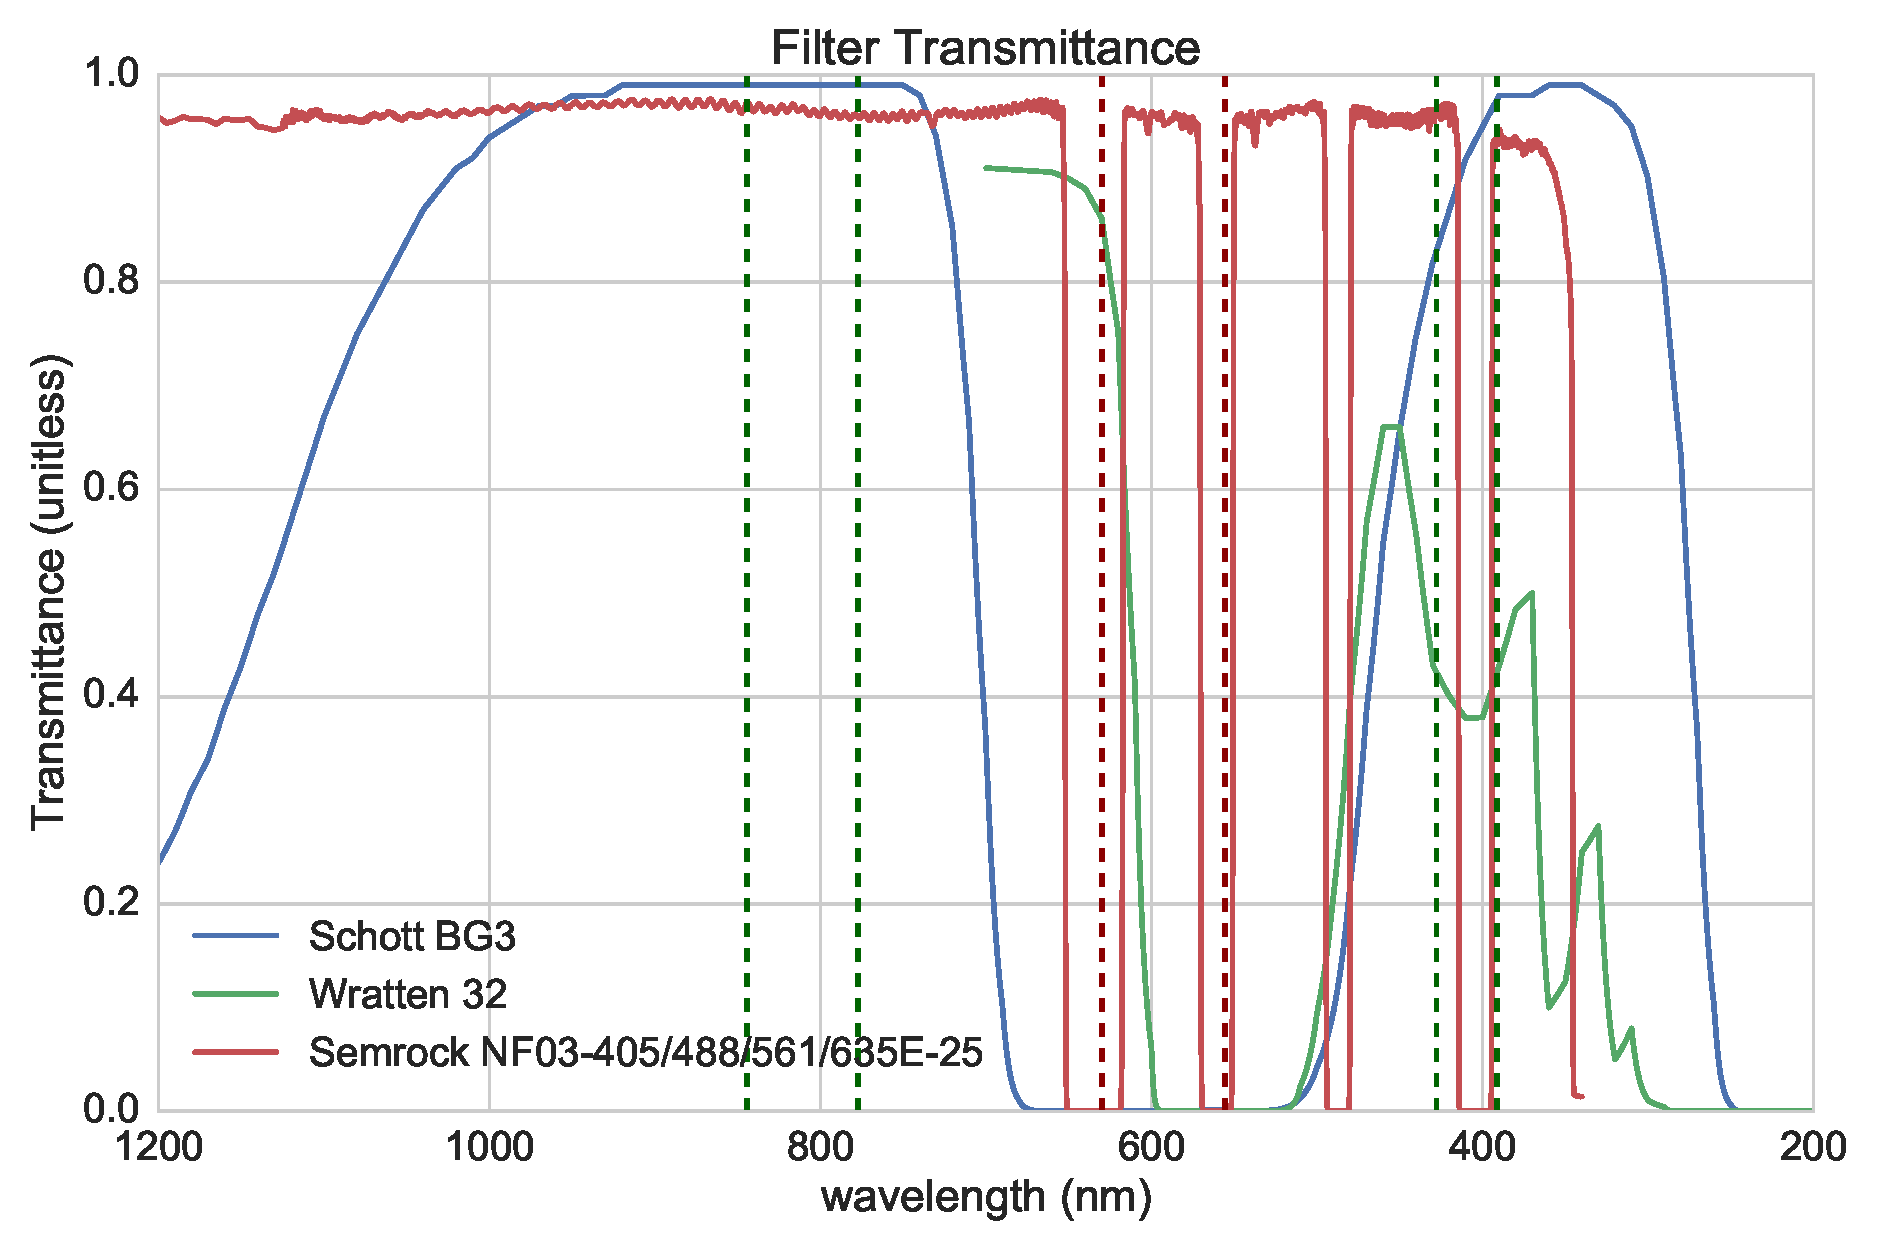
\includegraphics[width=0.9\columnwidth]{gfx/filterT}
    \caption{Comparison of bandstop filters used by other systems studying prompt auroral emissions with Schott BG3 bandstop filter used by HiST. Red markers at strong forbidden auroral emission wavelengths and green markers at strong permitted auroral emission wavelengths.}\label{fig:filters}
\end{figure}
The Wratten 32 filter \citep{wratten} has two deficiencies for fast auroral imaging: it passes the metastable oxygen emission at \unit[630]{nm} and has high attenuation of the NO emission at \unit[427.8]{nm}.
The Semrock NF03-405/488/561/635E-25 filter \citep{semrock} has similar performance \citep{jackel2014} for the auroral emissions of interest as the BG3 filters used for HiST.
HiST lenses yield a 9 degree field of view approximately centered on magnetic zenith, similar to the MOOSE instrument but HiST has significantly higher spatial resolution.
Star registration is via the astrometry.net software \citep{lang2010,hirschastro}, allowing a common local coördinate system to be created for PFISR and HiST \citep{geodata}.

The first considerations for designing a prompt auroral emissions observatory, whether based on ground, rocket or satellite include:
\begin{enumerate}
    \item Optical filtering: white light or no filtering will cover over prompt emissions with stronger, smeared forbidden emissions such as $\lambda = \unit[557.7]{nm}$, the first measured auroral emission line \citep{angstrom1869}.
    Shortpass filtering such as used in \citet{nishiyama2016} discards the medium brightness N$_2$ 1P \unit[670]{nm} and OI $\in \{777.4, 844.6\}$~nm emissions.
    Narrow-bandpass filtering discards most of the physical processes, leaving only part of the particle energy deposition picture available for estimation.
    HiST takes the bandstop filter approach, retaining most of the prompt emissions while discarding most forbidden emissions.
    \item Data inversion: remote observatories must either transmit or store data suitable for physical quantity estimation. HiST uses a unique implementation of model based iterative reconstruction (MBIR).
    MBIR reduces the dimensionality of difficult tomographic problems, thereby requiring less SNR for a given error level.
    In the medical field, MBIR is credited with reducing patient CT radiation doses by up to 98\% \citep{liu2014}.
    \item Data curation: MBIR estimation is known for being modestly time-consuming to compute.
    Currently, a single \unit[20]{ms} HiST frame takes about one minute to reconstruct a $\Phi_{top}(E,x)$ estimate \citep{hirsch2016}.
    To conserve human and computing resources, an on-site automatic data curation algorithm \citep{cviono} was developed and implemented \citep{hirsch2016bigdata}, allowing indefinite operating lifetime with yearly external USB 3.0 hard drive swap.
\end{enumerate}

Electron precipitation along $B_\parallel$ may be described by particle penetration models yielding wavelength-dependent optical intensity.
Auroral lines relevant to the filter selection of Figure~\ref{fig:filters} are listed in Table~\ref{tab:spectrum}.
\begin{table}\centering
    \caption{Selected auroral emission lines}\label{tab:spectrum}
    \begin{tabular}{rllll}
        \toprule
        $\lambda$ [nm] & family  & HiST system loss [dB] & lifetime [sec.] \\
        \midrule
        %297.2 &  [OI]31     & 13.5 & \\ % not visible due to O3 absorption (Chamberlain ch 5.1 p. 185)
        337.0 & N$_2^+$ 2P (0,0) &      &  \\
        % ~339.5 & N2+ 2P(3,6) \\
        391.4 & N$_2^+$ 1N (0,0) & 2.0  & $70 \times 10^{-9}$ \\ % high energy precip, V. Jones, 1971
        % ~394.3 & N2+ 2P(2,5) \\
        427.8 & N$_2^+$ 1N (0,1) & 1.7  & \\ % 25 R/nm
        470.9 & N$_2^+$ 1N & & \\
        486.1 & H$_\beta$ & & \\ % weak proton aurora 50-300R
        519.8, 520.0 & [NI]21 & & 1 day \\ % may be as strong as 557.7 forbidden (Chamberlain p.186)
        557.7 & [OI]32  (1s) & 28.9 & 0.74 \\ % 1190 R/nm  forbidden
        % 587.6 & He (3P-3D) & & \\ % rarely (P.E. Sandholt, Dayside and Polar Cap Aurora)
        % 589.0/589.6 & Na (2S-2P) & & \\ % occasionally (P.E. Sandholt, Dayside and Polar Cap Aurora)
        630.0 & [OI]21      & 49.7 & 107 \\  % 810R/nm forbidden
%        656.3 & H$_\alpha$ & & \\ % weak proton aurora 50-300R
        670.0 & N$_2$ 1P & &  \\ % prompt, NOT N2+
%        732.0,733.0 &    [OII] $^2$P-$^2$D & & \\ % 100eV, high altitude.  Sullivan et al
        750.0 & N$_2$ 1P & &  \\ % prompt, NOT N2+
        %761.9 &   &    & 0.9 \\ %not ground-visible: 02 absorption (Vallance Jones 1974)
        777.4 & OI   3s-3p  & 1.1 & \\  % low energy precip, quintet (chamberlain p.188) permitted
        844.6 & OI   3s-3p  & 2.3 & \\  % low energy precip, triplet permitted
        \bottomrule
    \end{tabular}
\end{table}
The temporal behavior along $B_\parallel$ help reveal the mechanism driving a particular auroral morphology.
\citet{hirsch2016} showed that using two or more tightly-synchronized high-speed cameras separated by \unit[1..10]{km} and co-aimed at magnetic zenith has high spatio-temporal resolution without the inherent ambiguities of \textit{a priori} starting altitude made necessary in single-camera studies.
Thus, DAW and inverted-V aurora for discrete arcs, even closely $B_\perp$-spaced arcs can be distinguished with HiST.

Based on rocket measurement and theory, fine spatio-temporal $B_\perp$ auroral structure comes from DAW.
HiST analysis uses a physics-based ionospheric forward model for electron precipitation in the \unit[50]{eV}..\unit[18]{keV} range with two high-speed cameras spaced \unit[3]{km} apart.
Model-based iterative reconstruction is used to estimate the differential number flux of the particles versus space and time at the top of the ionosphere.
We define the top of the ionosphere as the region below which particle acceleration is neglected and above which energy deposition is neglected.
In this manner, tightly time-synchronized camera data at \unit[30]{ms} cadence combined with ISR measurements at \unit[100]{ms} cadence yield confirming evidence for the association of DAW with strong turbulence in the lower ionosphere.

The phase 1 HiST \unit[30]{ms} observational cadence is fast enough \citep{peticolas2000,hirsch2016} to observe signatures of DAW-accelerated particle precipitating into the ionosphere.
As implied by the name, dispersive acceleration leads to higher energy particles arriving at the ionosphere first, and therefore depositing their energy in the E-region ionosphere before the lower energy particles of the same magnetospheric particle batch arrive.
The time delay between high and low energy particles is only a few hundred milliseconds \citep{dahlgren2013}, so the HiST sampling cadence gives several estimates of auroral precipitation characteristics during a dispersive impulse, sufficient to resolve key parameters of the event such as characteristic energy and beam location versus time \citep{histfeas}.


\FloatBarrier
\subsection{PFRR Digital Meridian Scanning Photometer (PDMSP)}\label{sec:pdmsp}
P-DMSP collects a six-wavelength view of intensity vs. elevation and time along the local magnetic meridian.
The meridional intensity is measured for wavelengths $\lambda \in \lbrace 427.8, 486.1, 520.0, 557.7, 630.0, 670.0 \rbrace$~nm.
The typical measurement cadence is 14 seconds, so this measurement is contextual and secondary to the primary HiST and PFISR measurements \citep{meridianreader}.
Although HiST cadence is nearly three orders of magnitude faster than P-DMSP, the spectrometer nonetheless provides temporally smeared spectral context over a wide elevation range.
A future deployment of HiST is expected to include an EMCCD-based spectrograph operating at a comparable frame rate to the full-frame HiST EMCCD imagers.
\section{Results}\label{sec:fusana}

Discrete auroral drivers can be broadly divided into quasi-static inverted-V structures and Alfvén waves (AW).
AW-driven auroral forms include splitting auroral arcs and flaming aurora.
Discrete auroral arcs driven by sources other than dispersive Alfvén waves include kinked auroral arcs and non-flaming, non-splitting discrete arcs.
HiST can distinguish between the differential number flux precipitation signatures responsible for AW and non-AW aurora.

Inverted-V potential drops have several associated mechanisms that can lead to fast time-dependent behavior such an intensity modulation.
Inverted-V auroral features do not have dispersive energy behaviors associated with them--precipitating particles across a range of energies arrive at roughly the same time $\Delta t \ll \unit[10]{ms}$ difference.
Double layers, and series of double layers may exist within an inverted-V structure giving rise to narrower width auroral arcs.

AW are associated with reconfiguration of the magnetosphere--particularly during the breakup and expansion phase of substorms, where a quarter-trillion watts are launched towards Earth \citep{mottez2015}.
AW are integral to the settling out of the system after a change in current flux.
The conditions favorable for DAW aurora are delineated in Figure~\ref{fig:alfvenblock}.
\begin{figure}\centering 
    %the \par is necessary after each text to make the \baselineskip take effect
    \begin{tikzpicture}[node distance=1.5cm, auto]
    
    \node (magdis) [startstop,text width=4cm] {Magnetospheric discontinuity (e.g. reconnection) \par };
       
    \node (iaw) [process, below of = magdis,xshift=-1 cm] {IAW $B_\parallel$ \par };
    
    \node (kaw) [process,right of = iaw,xshift=1 cm] {KAW $B_\parallel$ \par };
    
    \node (wl) [decision, below of=iaw,text width=2 cm,yshift=-0.75cm] { cold plasma  $\omega < \omega_{ci}$ $v_A > v_{te}$ \par };
    
    
    \node (iontherm) [estimate, below of=wl,yshift=-1 cm, text width=5cm]{ $k \sim$ ion thermal gyroradius: $ \rho_i = \frac{\sqrt{T_i/m_i}}{\omega_{ci}} $ \par};
    
    \node (iongyro) [estimate, left of=iontherm,xshift=-4cm, text width=4cm]{ $k \sim$ ion gyroradius: $ \rho_s = \frac{\sqrt{T_e/m_i}}{\omega_{ci}} $ \par};
    
    \node (eskin) [estimate, right of=iontherm,xshift=4cm,text width=4cm]{ $k \sim$ electron skin depth: $\lambda_e = \frac{c}{\omega_{pe}}$ \par};
    
    \node (accel) [process, below of=iontherm,yshift=-0.25cm]{$ E_\parallel$ \par};
    
    \node(eflux) [process,below of=accel,text width=4cm]{100x background dispersive or flat-top electron flux $\Phi$ \par};
    
    \node(lt) [startstop, below of=eflux,xshift=-2cm]{Langmuir Turbulence \par};
    
    \node(aurora) [startstop, below of=eflux,xshift=2cm]{Alfvénic Aurora \par};
    
    \node(neial) [compute,below of=lt,xshift=-1cm] {NEIALs \par};
    \node(isr) [compute,below of=neial]{ISR backscatter \par};
    \node(isrest)[startstop,below of=isr,text width=3cm,yshift=-.5cm]{CFAR Turbulence estimate \par};
    
    \node(hist)[compute,below of=aurora,xshift=1cm]{HiST: filter, camera};
    \node(det)[compute,below of=hist,text width=3cm,yshift=-.5cm]{HiST: Alfvénic discrimination algorithm};
    \node(est)[startstop,below of=det,text width=3cm,yshift=-.75cm]{HiST: $\Phi_{top}$ precipitation estimation};
    
    \draw[arrow] (magdis) -- (iaw);
    \draw[arrow] (magdis) -- (kaw);
    \draw[arrow] (iaw) -- (wl);
    \draw[arrow] (wl) -- (iongyro);
    \draw[arrow] (wl) -- (iontherm);
    \draw[arrow] (wl) -- (eskin);
    \draw[arrow] (iongyro) -- (accel);
    \draw[arrow] (iontherm) -- (accel);
    \draw[arrow] (eskin) -- (accel);
    \draw[arrow] (accel) -- (eflux);
    \draw[arrow] (eflux) -- (aurora);
    \draw[arrow] (eflux) -- (lt);
    
    \draw[arrow] (lt) -- (neial);
    \draw[arrow] (neial) -- (isr);
    \draw[arrow] (isr) -- (isrest);
    
    \draw[arrow] (aurora) -- (hist);
    \draw[arrow] (hist) -- (det);
    \draw[arrow] (det) -- (est);
    
    \end{tikzpicture}
    \caption{Block diagram of Alfvénic aurora acceleration mechanism and HiST observation.}
    \label{fig:alfvenblock}
\end{figure}
A key ground-observable characteristic of Alfvénic aurora is narrow arc width.
``Width'' describes spatial scale size in the dimension perpendicular to geomagnetic field $B$.
\citet{maggsdavis1968} noted that the lower observed limit of \unit[70]{m} arc width was instrumentally limited.
\citet{borovsky1993} noted that observations from contemporary ground-based auroral arc measurements continued to reveal arc widths less than \unit[100]{m}.
Alfvénic aurora are associated with a sudden large increase in flux of particles accelerated from a few eV to as much as \unit[10]{keV} \citep{chaston2003}.
Due to dispersion along the accelerated particle path, over several hundred milliseconds \citep{dahlgren2013} the characteristic energy $E_0$ will go from order \unit[10]{keV} to order \unit[100]{eV}.
A representative differential number flux for a DAW event is shown in Figure~\ref{fig:alfvenflux}.
\begin{figure}
    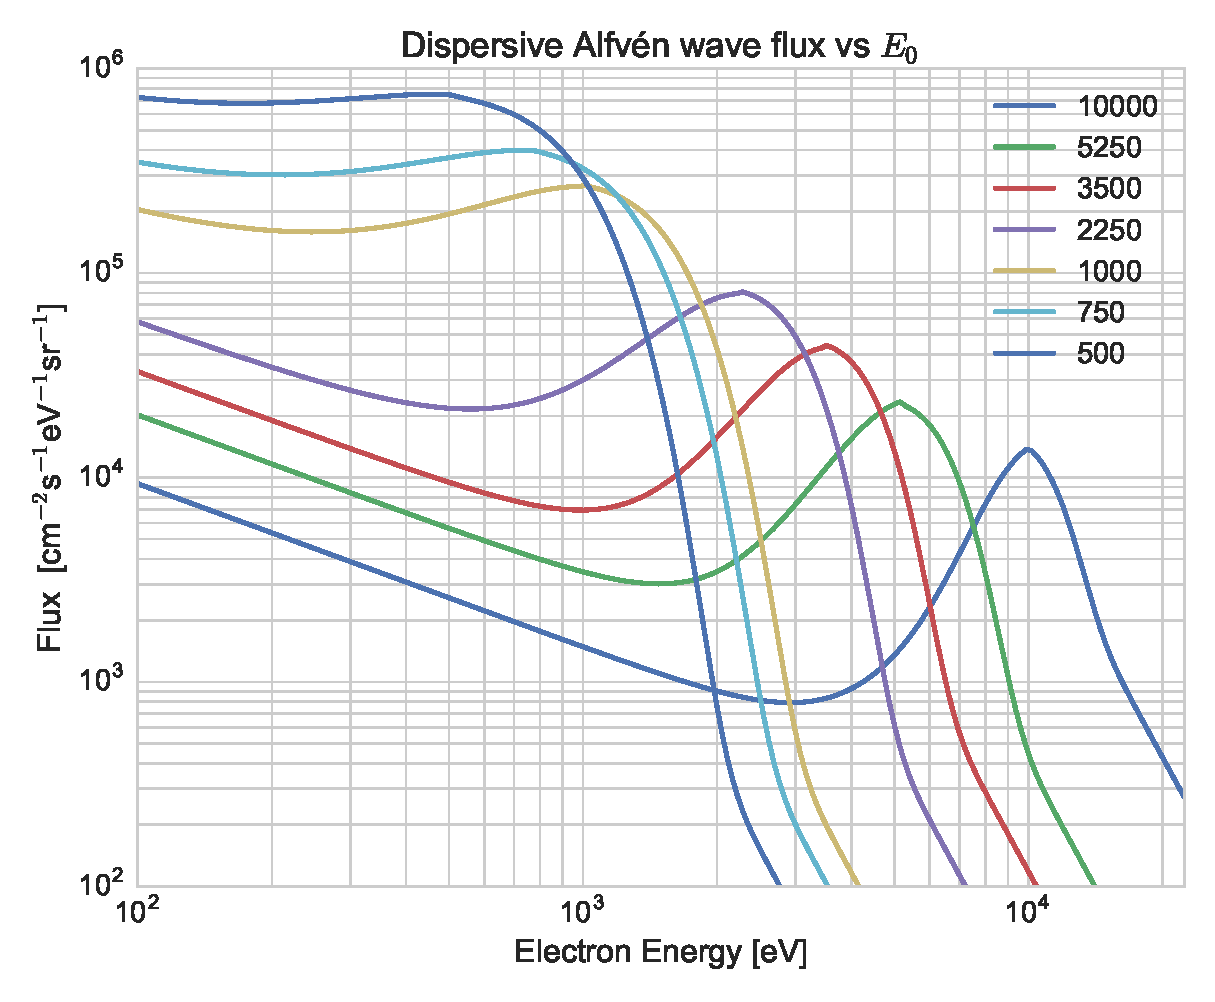
\includegraphics[width=0.9\columnwidth]{gfx/eflux}
    \caption{Evolution of characteristic energy $E_0$ from order \unit[10]{keV} to order \unit[100]{eV} occurs in \unit[100..1000]{ms} for DAW.
    In this plot, overall flux $Q_0$ is held constant.}
    \label{fig:alfvenflux}
\end{figure}
\textit{In situ} Freja measurements with \unit[32]{kHz} sampling rate \citep{stasiewicz2000} consistently showed plasma evacuations by roughly a factor of two near magnetic perturbations along $B_\parallel$ consistent with the presence of Alfvén waves.
Considering the \unit[7]{km/s} platform motion, the spectrograms of magnetic field point to $k_\perp \in [10,7000]$~m.
Freja also observed clear correlations \citep{stasiewicz2000} with turbulent magnetic field and suprathermal electron bursts ranging from \unit[100]{eV} to \unit[20]{keV} with particle fluxes of order 100 times over the background, and Poynting flux of $\unit[1..20]{mW/m^2}$.

The sampling cadence configuration of PFISR and the optical instruments for each experiment is given in Table~\ref{tab:cadence}.
These raw sample times are far faster than the minute cadence typically employed for plasma parameter estimation, yet those minute-long estimates break down in the face of these transient events.
We examine four types of events in turn: auroral breakup, splitting auroral arc, flaming auroral arc, and kinked arc with joint analysis of optical, spectral and radar features.


\FloatBarrier
\subsection{Breakup Auroral Arcs}\label{sec:breakup}
Highly dynamic events may combine several auroral morphologies, driven by diverse acceleration mechanisms, yielding multiple plasma turbulence types in close spatiotemporal proximity.
These events are difficult to interpret with instruments smearing in time by a factor of 100..1000 times greater than the ground-observable timescales.
It is also impractical to have a human manually initiating recording during extended observations.
This fact motivates the automatic Alfvénic aurora discrimination algorithms cited in section~\ref{sec:hist}.

A canonical example of such an event motivating the HiST system was the auroral breakup of March 23, 2007 shown in Figure~\ref{fig:20070323}.
\begin{figure}
    \noindent\includegraphics[width=0.9\columnwidth,trim=0 383 0 10,clip]{gfx/2007-03-23/2007-03-23}
    \vspace{0.1cm}
    
    % psd ion-line
    \includegraphics[width=0.3\columnwidth,trim=0 55 0 0]{gfx/2007-03-23/acfslice_alternatingcode2007-03-2311-20-08}
    \includegraphics[width=0.3\columnwidth,trim=0 55 0 0]{gfx/2007-03-23/acfslice_alternatingcode2007-03-2311-20-23}
    \includegraphics[width=0.3\columnwidth,trim=0 55 0 0]{gfx/2007-03-23/acfslice_alternatingcode2007-03-2311-20-39}
    
    \vspace{-0.5cm}
    \hspace{0.1cm}(f)\hspace{0.275\columnwidth}(g)\hspace{0.275\columnwidth}(h)
    \vspace{0.1cm}
    
    % psd plasma-line
    \includegraphics[width=0.45\columnwidth,trim=0 60 0 0]{gfx/2007-03-23/plasmaDOWNslice2007-03-2311-20-08}
    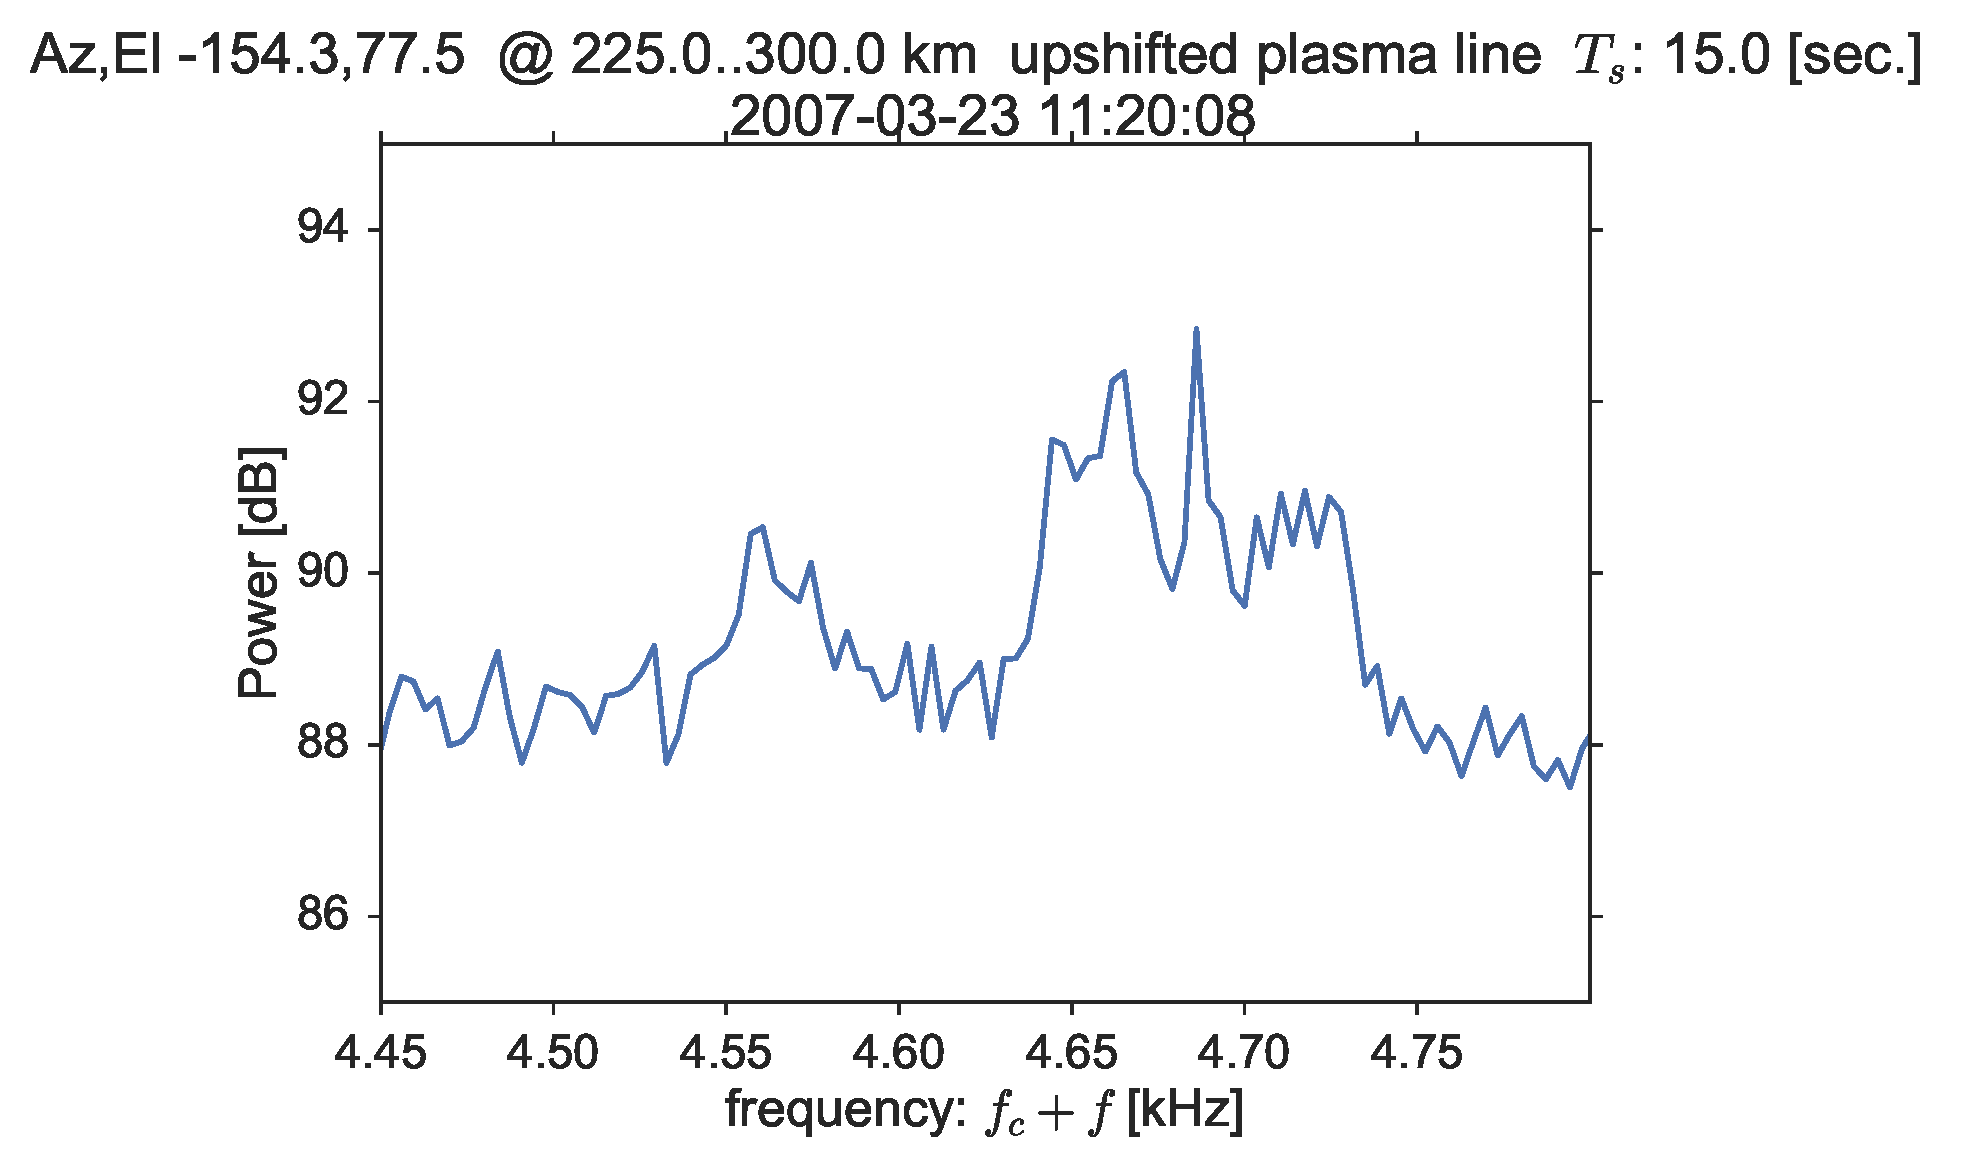
\includegraphics[width=0.45\columnwidth,trim=0 60 0 0]{gfx/2007-03-23/plasmaUPslice2007-03-2311-20-08}
    
    \vspace{-0.5cm}
    \hspace{0.5cm}(i)\hspace{0.425\columnwidth}(j)
    \vspace{0.5cm}
    
    \caption{Substorm breakup: highly dynamic aurora on 23 March 2007. 
        Low-altitude NEIALs observed corresponding to (a,c,f,i,j) with possible Farley-Buneman instability in the E-region. 
        Streaming upflow corresponding to (d,h).
    Strong Langmuir turbulence corresponding to (c,f,g). }\label{fig:20070323}
\end{figure}
The PF-DMSP spectra ratio $I_{6300}/I_{4278}$ in Figure~\ref{fig:mspratio0323} dips as low as 0.02 during the breakup, indicating a large flux with $E_0 > \unit[10]{keV}$ according to \citet{rees1974}.
\begin{sidewaysfigure}\centering
    \includegraphics[width=0.85\linewidth]{gfx/2007-03-23/msp-ratio}
    \caption{PF-DMSP spectral ratio breakup event 2007 March 23 11:22 UTC.
        The ratio $I_{6300}/I_{4278}$ dips as low as 0.02 during the breakup, indicating a large flux with $E_0 > \unit[10]{keV}$ according to \citet{rees1974}.}
    \label{fig:mspratio0323}
\end{sidewaysfigure}
The $I_{5577}/I_{4278}$ in Figure~\ref{fig:mspratio0323-5577} dips as low as 1 during the breakup, also indicating a large flux with $E_0 > \unit[10]{keV}$ according to \citet{rees1974}.
\begin{sidewaysfigure}\centering
    \includegraphics[width=0.85\linewidth]{gfx/2007-03-23/msp-ratio-5577}
    \caption{PF-DMSP spectral ratio breakup event 2007 March 23 11:22 UTC.
        The ratio $I_{5577}/I_{4278}$ dips as low as 1 during the breakup, indicating a large flux with $E_0 > \unit[10]{keV}$ according to \citet{rees1974}.}
    \label{fig:mspratio0323-5577}
\end{sidewaysfigure}
The GIMA magnetometers data surrounding this event is shown in Figure~\ref{fig:20070323mag}, with the expected strong perturbation near the event time.
\begin{figure}
    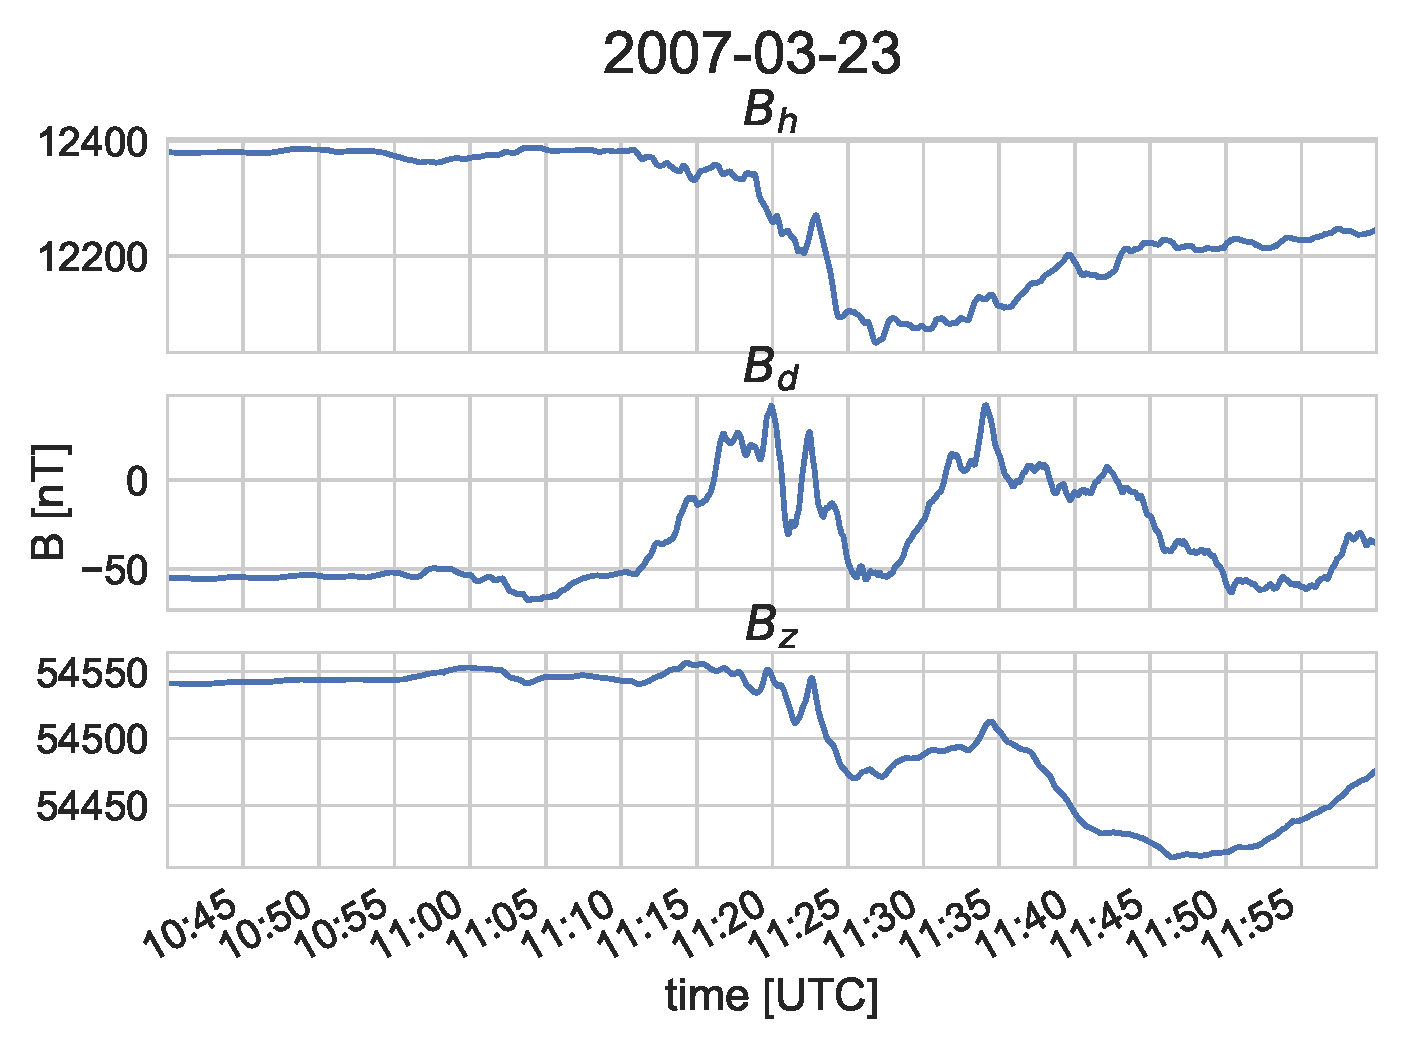
\includegraphics[width=\columnwidth]{gfx/2007-03-23/mag}
    \caption{Strong B-field perturbance due to substorm on 2007-03-23 near 11:20 UTC.}
    \label{fig:20070323mag}
\end{figure}

This was an exceptionally intense breakup event.
This magnificent substorm breakup had splitting arcs embedded in the wildly dynamic behavior captured by PFISR and a single BG3-filtered EMCCD camera. 
This event has been analyzed in detail by \citet{semeter2008,akbari2012}.


\subsection{Splitting Auroral Arcs}\label{sec:split}
One of the ground-observable optical manifestations of a DAW event are bifurcating ``shedding'' or ``splitting'' arcs, which have a pattern of one or more spatiotemporal leaves folding off of the main arc. 
During the shedding event of Figures~\ref{fig:20130414T0854a}-\ref{fig:20130414T0854b}, PFISR power in the magnetic zenith beam (represented by a red circle in Figure~\ref{fig:20130414T0854a}(a-d)) is enhanced by over \unit[25]{dB} in the F-region ionosphere above the bifurcation zone.
\begin{sidewaysfigure}\noindent

    \includegraphics[width=\columnwidth,trim=0 680 0 50,clip]{gfx/2013-04-14T0854/2013-04-14T0854}\\
    
    \vspace{-1.175cm}
    \hspace{1.35cm}{\color{white}(a) 08:54:16}
    \hspace{2.1cm}{\color{white}(b) 08:54:21}
    \hspace{2.15cm}{\color{white}(c) 08:54:26}
    \hspace{2.15cm}{\color{white}(d) 08:54:31}
    \vspace{0.5cm}
    
    % backscatter
    \begin{center}
    \includegraphics[width=0.9\columnwidth,trim=10 0 0 185,clip]{gfx/2013-04-14T0854/power_longpulse2013-04-1408-54}\\
    \end{center}
    
    \vspace{-1.5cm}
    (e) 
    \vspace{.5cm}
      
    \caption{Splitting auroral arc sequence at PFISR, April 14, 2013. 
        (a) beginning of plasma turbulence bursts.
        (b) F-region ionization increasing nearly \unit[30]{dB} above background. 
        The turbulence fades in (c), enhancing to even greater intensity in (d) for ten seconds.
        (e) backscattered ISR power.}
    \label{fig:20130414T0854a}
\end{sidewaysfigure} 

\begin{figure}\noindent
	   % psd ion-line 
	\includegraphics[width=0.425\columnwidth]{gfx/2013-04-14T0854/acfslice_longpulse2013-04-1408-54-16}
	\includegraphics[width=0.425\columnwidth]{gfx/2013-04-14T0854/acfslice_longpulse2013-04-1408-54-31}\\
	
	\vspace{-1.5cm}
	\hspace{0.0cm}(a)\hspace{0.4\columnwidth}(b)
	\vspace{0.3cm}
	
	% down-shift
	\includegraphics[width=0.425\columnwidth,trim=0 50 0 0]{gfx/2013-04-14T0854/plasmaDOWNslice2013-04-1408-54-16}
	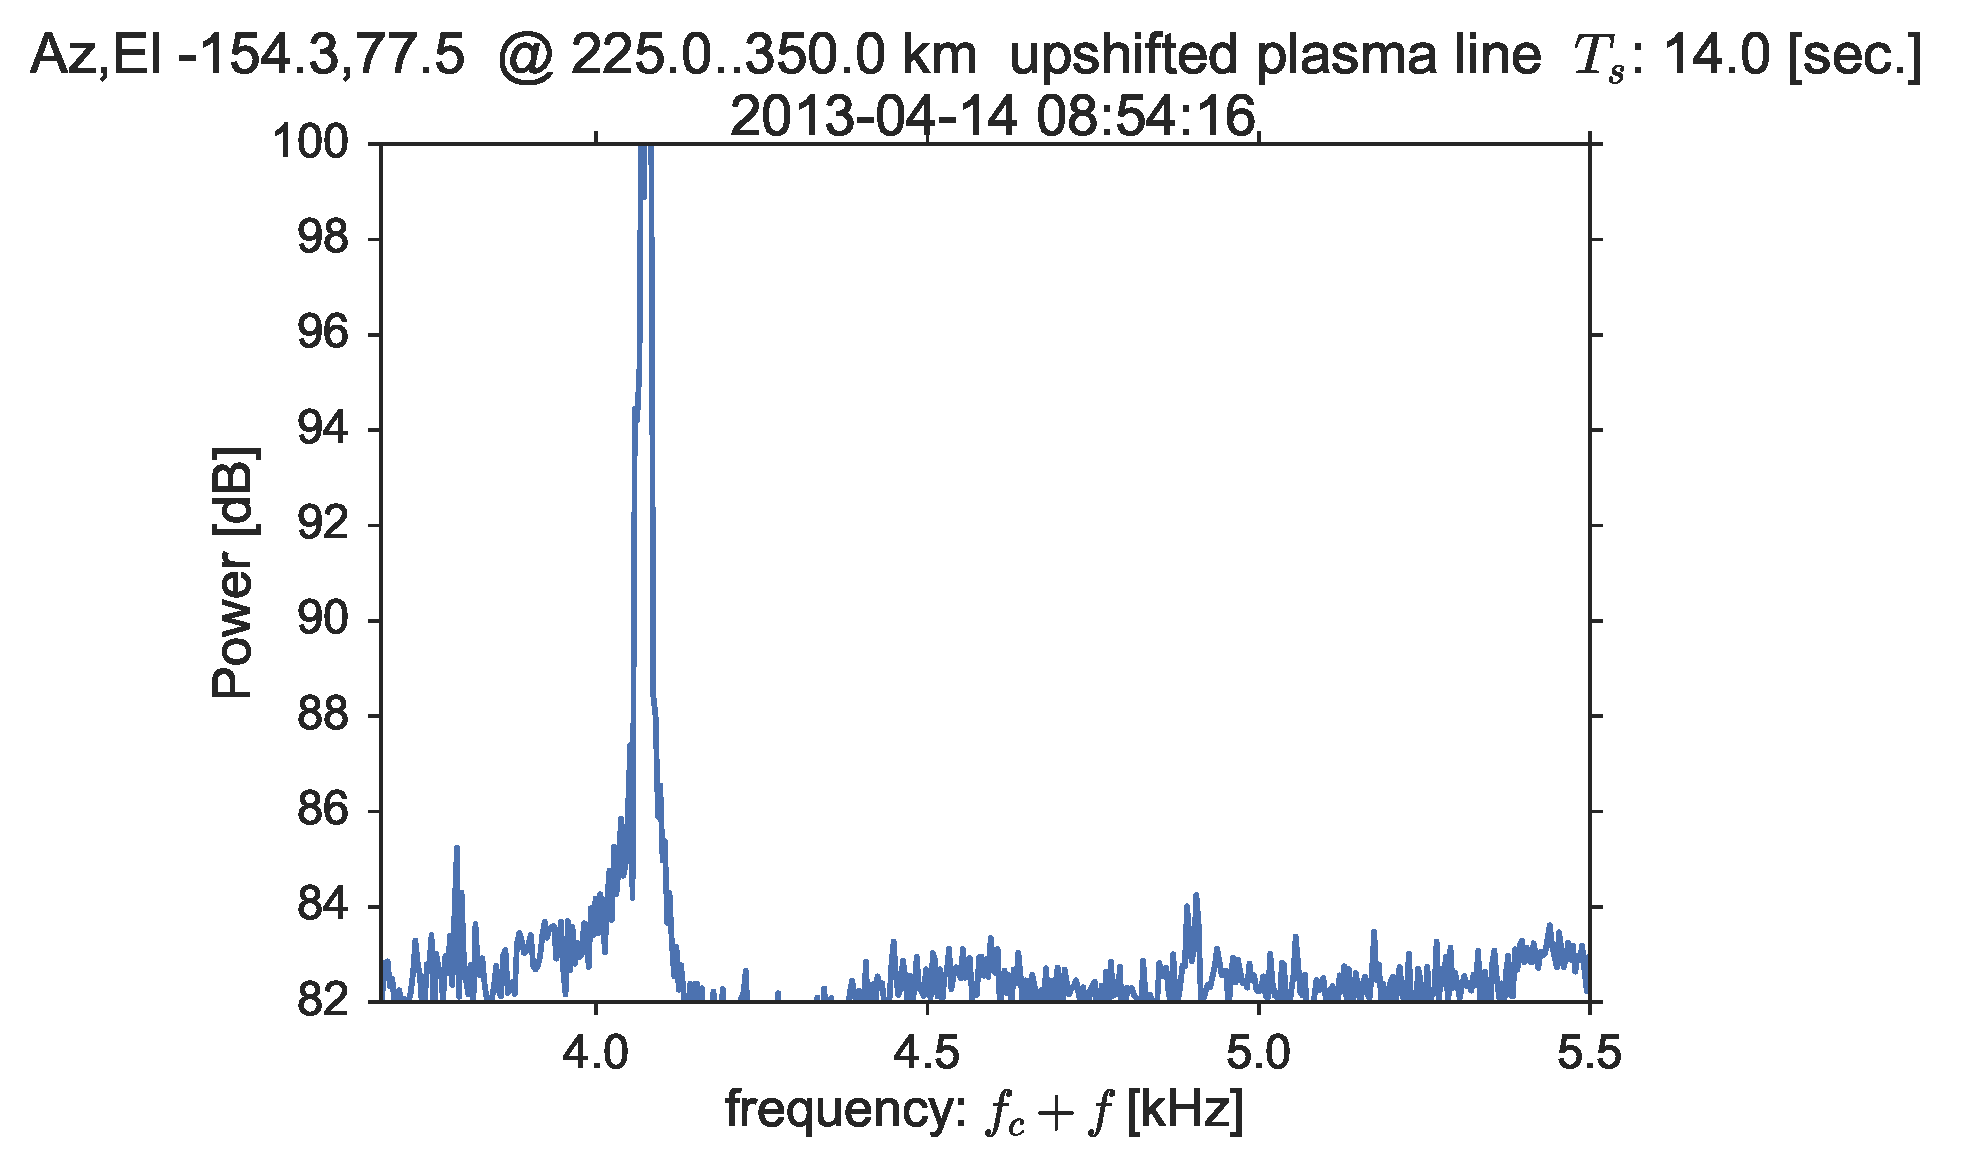
\includegraphics[width=0.425\columnwidth,trim=0 50 0 0]{gfx/2013-04-14T0854/plasmaUPslice2013-04-1408-54-16}\\
	
	\vspace{-1.2cm}
	\hspace{0.0cm}(c)\hspace{0.4\columnwidth}(d)
	\vspace{0.3cm}
	
	% up-shift
	\includegraphics[width=0.425\columnwidth,trim=0 50 0 0]{gfx/2013-04-14T0854/plasmaDOWNslice2013-04-1408-54-31}
	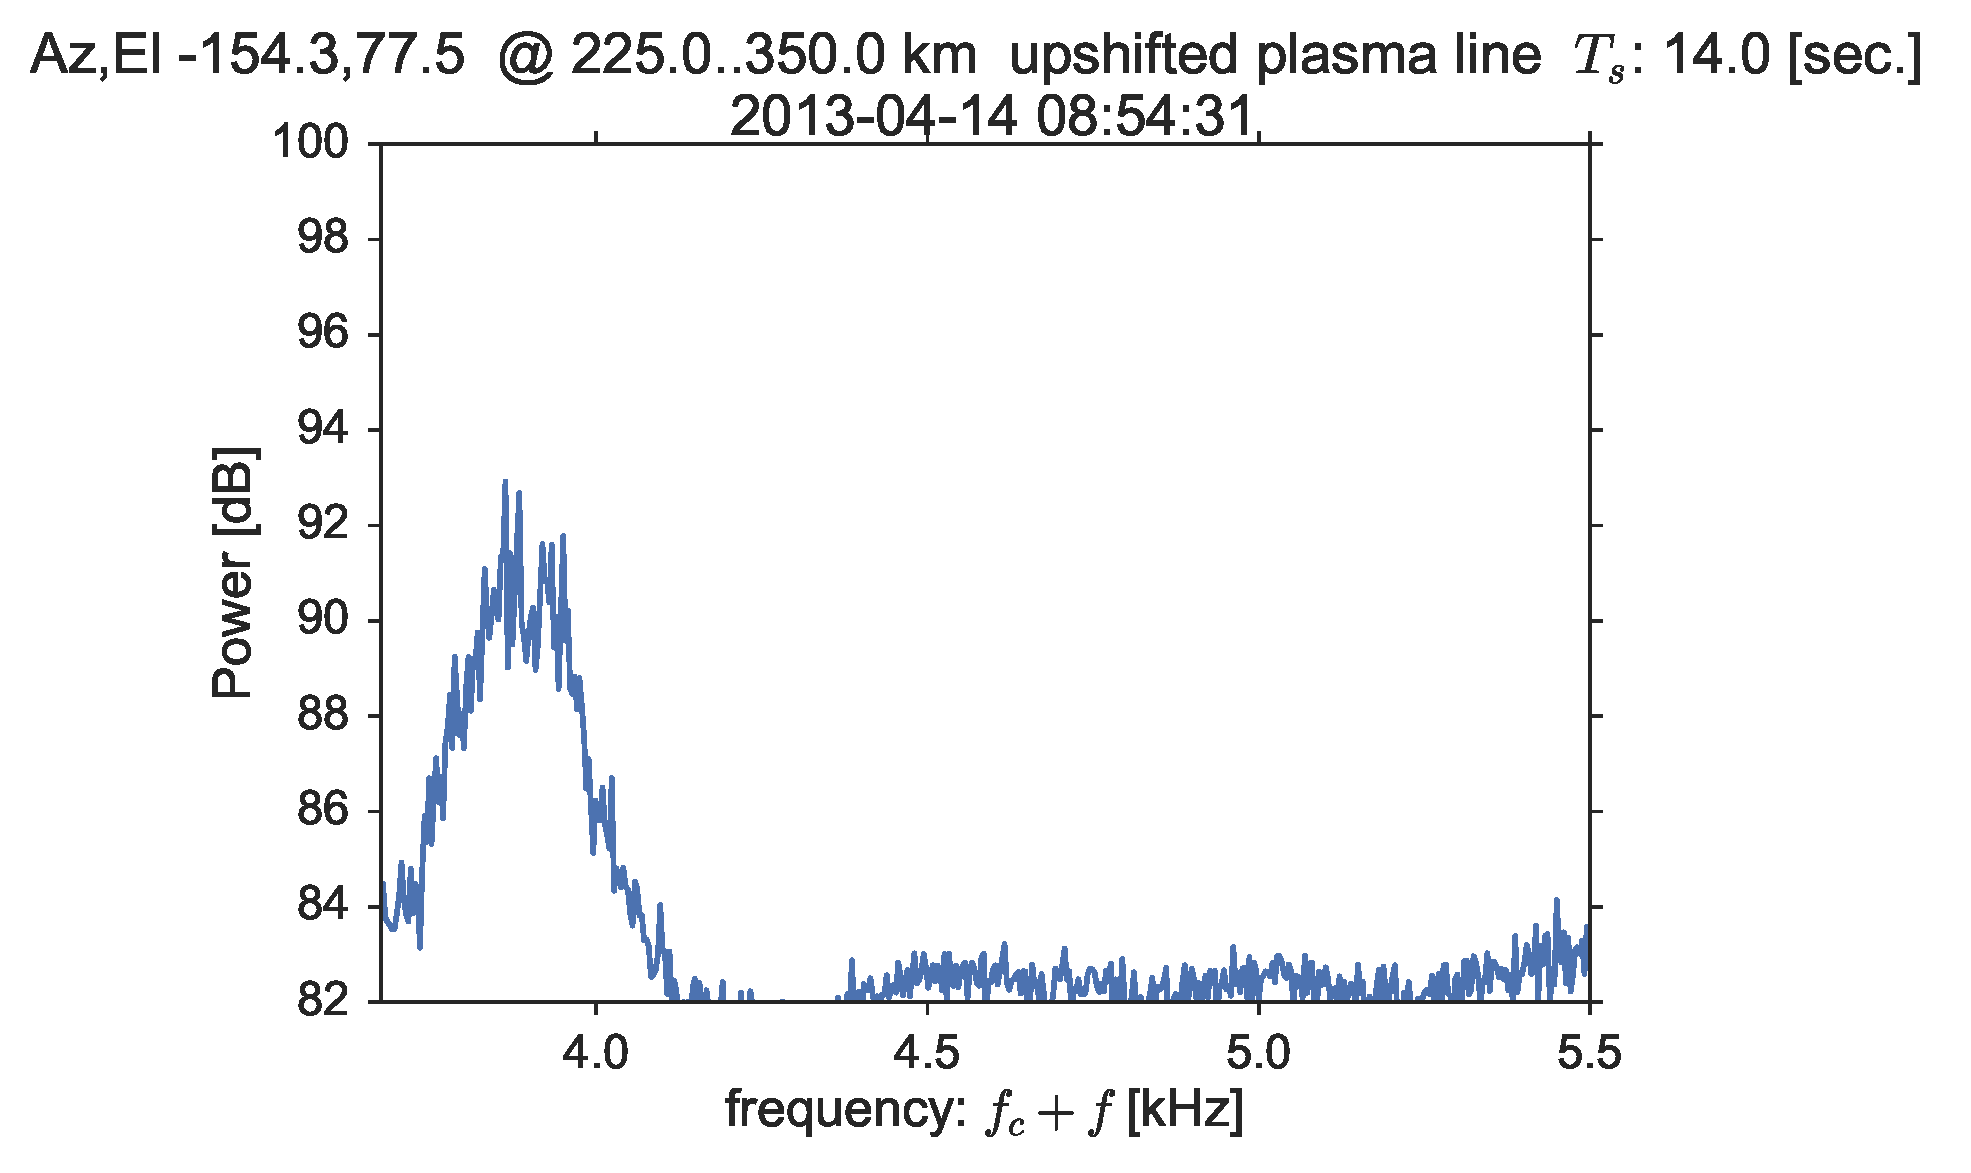
\includegraphics[width=0.425\columnwidth,trim=0 50 0 0]{gfx/2013-04-14T0854/plasmaUPslice2013-04-1408-54-31}\\
	
	\vspace{-1.2cm}
	\hspace{0.0cm}(e)\hspace{0.4\columnwidth}(f)
	\vspace{0.3cm}
	
	\caption{Splitting auroral arc sequence at PFISR, April 14, 2013.
		(a,b) backscattered power related to (a-c) and (d) respectively.
		(c,d) down- and up-shifted plasma line enhancements corresponding to Figure~\ref{fig:20130414T0854a}(a-c).
		(e,f) down- and up-shifted plasma line enhancements corresponding to Figure~\ref{fig:20130414T0854a}(d).}
	\label{fig:20130414T0854b}
\end{figure}
On the night of April 14, 2013, several instruments with diverse observing modalities were active in the vicinity of PFRR, as depicted in Figure~\ref{fig:sitemap}. 
PFISR and DASC are co-located, so the center of the PFISR beams in the image can be taken as approximately constant.
The GIMA magnetometer data is shown in Figure~\ref{fig:gima0854}, showing the usual southward IMF in the time vicinity of the splitting arc.
\begin{figure}
	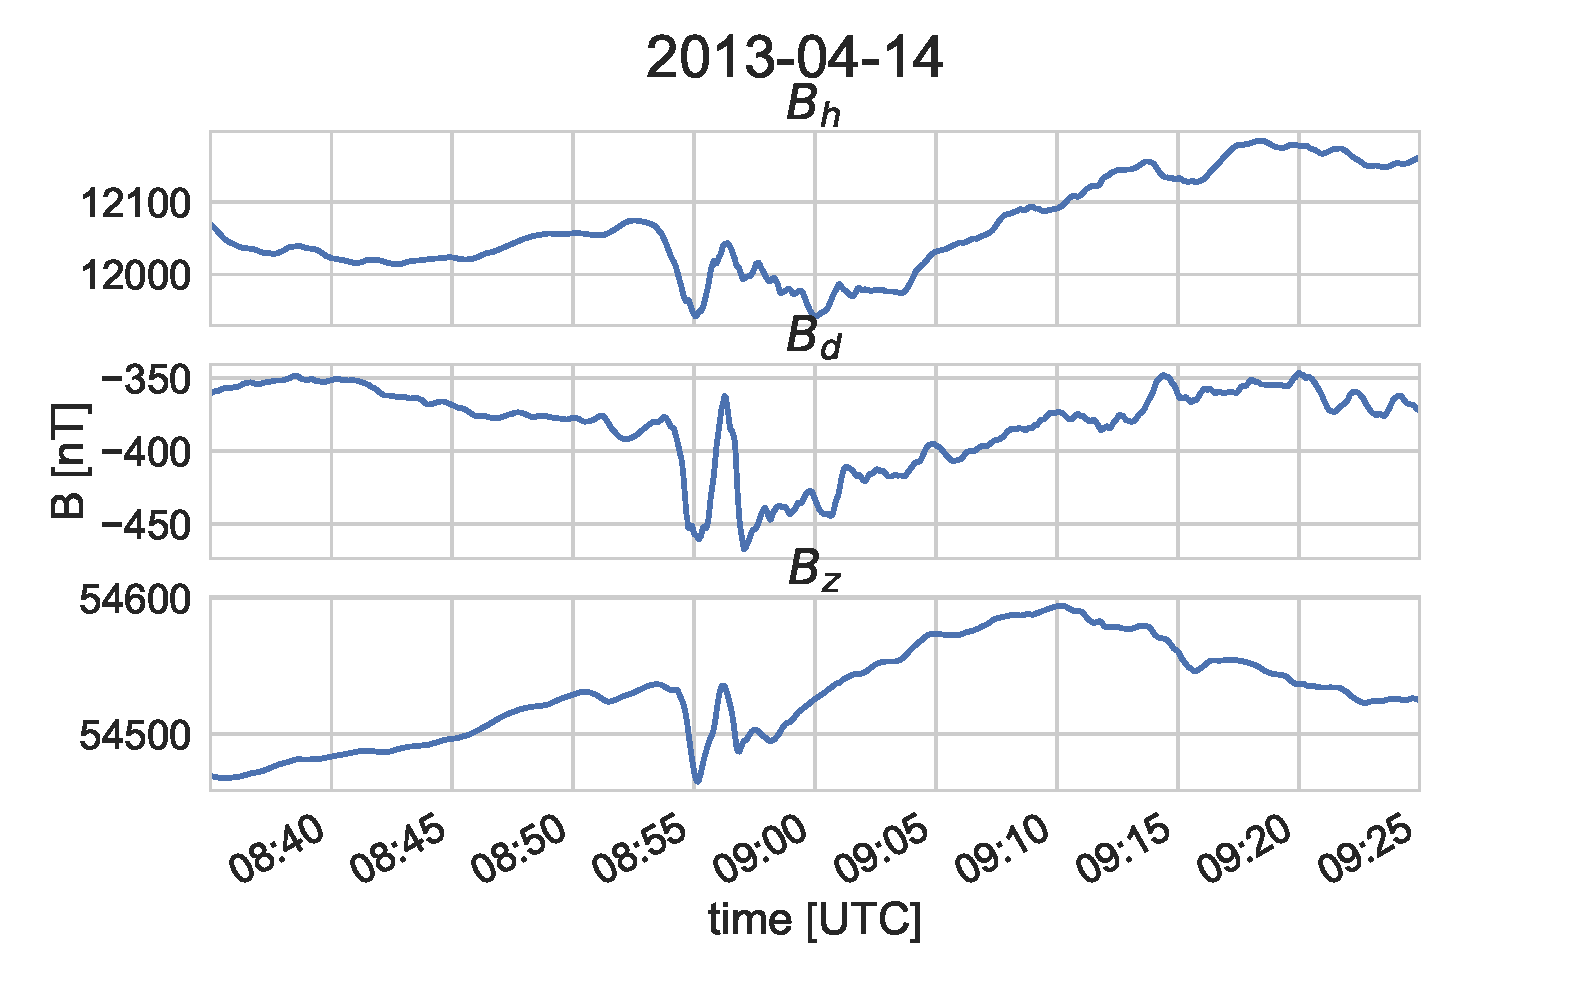
\includegraphics[width=\columnwidth]{gfx/2013-04-14T0854/mag}
	\caption{PFRR GIMA magnetometer data for 2013-04-14 showing evidence of southward IMF in time vicinity of splitting arc.}
	\label{fig:gima0854}
\end{figure}


Observe in Figure~\ref{fig:20130414T0854b}(c-f) that only the plasma line spectra for 08:54:16 and 08:54:31 UT show prominent reflections from plasma turbulence.
The rest of the plasma line spectra near this time looks much like the 08:54:45 data.
%In contrast, the ion line spectrum in Figure~\ref{fig:20130414T0854}(f,g,h) still shows the turbulence effects at 08:54:45, so an earlier frame at 08:54:02 UT is included to show the non-turbulent ion line spectra.
%A movie sequence for this event is available in the Supplemental Materials for this article.
We integrate the received ISR power over the NEIALs altitude range and plot this integrated measurement with the HiST optical data. 
It is initially apparent from comparing Figure~\ref{fig:20130414T0854a}(a-d) with Figure~\ref{fig:20130414T0854a}(e) that the highest SNR bursts come from the times when the magnetic zenith ISR beam is over a region of optically ``shedding'' arcs.
Figure~\ref{fig:20130414T0854a}(a) depicts a typical dispersive Alfvén wave auroral scene. 
The red circle denotes local magnetic zenith. 
Observe the fine spatial structure along the $B_\perp$ direction. 
Figure~\ref{fig:shedintion}(b) shows the plasma line summed over altitudes from \unit[200..350]{km}.
Figure~\ref{fig:20130414T0854b}(a,b) shows the ion line PSD during the time of this shedding auroral event--observe the ``flat top'' characteristic of the spectrum seen only during NEIALs.

Turning to optical spectral information, the PF-DMSP data in Figure~\ref{fig:shedratio0854}(a-b) is used to compare \unit[427.8]{nm} intensity from N$_2^+$ $I_{427.8}$ with prompt OI emissions at \unit[630.0]{nm} $I_{630.0}$.
This ratio in Figure~\ref{fig:shedratio0854}(c) shows that just before and during the splitting arc, $I_{427.8}$ is nearly twice as strong as $I_{630.0}$. 
\begin{figure}
    \includegraphics[width=\columnwidth,trim=3 3 3 3,clip]{gfx/2013-04-14T0854/MSPintensityratio}
    \caption{PF-DMSP (a) $I_{630.0}$ and (b) $I_{427.8}$ emission intensity with (c) $I_{630.0}/I_{427.8}$ emission intensity ratio at 08:54 UT during the 14 April 2013 substorm. Golden dashed lines refer to approximate elevation FOV of HiST cameras.}\label{fig:shedratio0854}
\end{figure}
After the splitting event completes, the \unit[630.0]{nm} line once again dominates $I_{427.8}$ by a factor of 1.5 to 3.5 as was also the case before the splitting began.
Figure~\ref{fig:shedratioplot0854} provides an alternative view of $I_{630.0}$/$I_{427.8}$.
\begin{figure}
    \includegraphics[width=0.9\columnwidth]{gfx/2013-04-14T0854/msp_ratio}
    \caption{PF-DMSP ratio of $I_{630.0}/I_{427.8}$ emission intensity ratio with one line plot per time. Observe that high energy beam (indicated by lowest ratio at 08:54:10) does not immediately lead to splitting arc. It takes about 10 seconds for visible arc splitting to occur. Golden dashed lines refer to approximate elevation FOV of HiST cameras.}
    \label{fig:shedratioplot0854}
\end{figure}
%These measurements are within the typical range for $I_{630.0}$ and $I_{427.8}$~\citep{Dashkevich2006}.
From \citet{rees1974}, at 08:54:10 UTC at the magnetic zenith angle of $102.5^\circ$ elevation from north, $I_{630.0}/I_{427.8} \sim 0.6$, corresponding to a characteristic energy of \unit[1.6]{keV} for the assumptions on neutral composition and brightness observed.

Historical work has often relied on spectrometer readings for estimates of characteristic energy $E_0$, represented in Figure~\ref{fig:alfvenflux} as the high-energy ``bump''.
Historically these measurements had cadences of several seconds, and obviously lacked a sense of the auroral morphology.
As the extensive literature referenced throughout this paper has noted, quantitative correlation of auroral spatio-temporal evolution with plasma turbulence requires an FOV of several degrees about magnetic zenith with at least 40 frames/s sampling, and with filtering sufficient to remove the blur of metastable emissions \citep{hirsch2016}.
The tomography data inversion exemplified in Figures~\ref{fig:histfwd} and \ref{fig:histest} is an example of the new capabilities afforded by HiST for such applications.
\begin{sidewaysfigure}\centering
    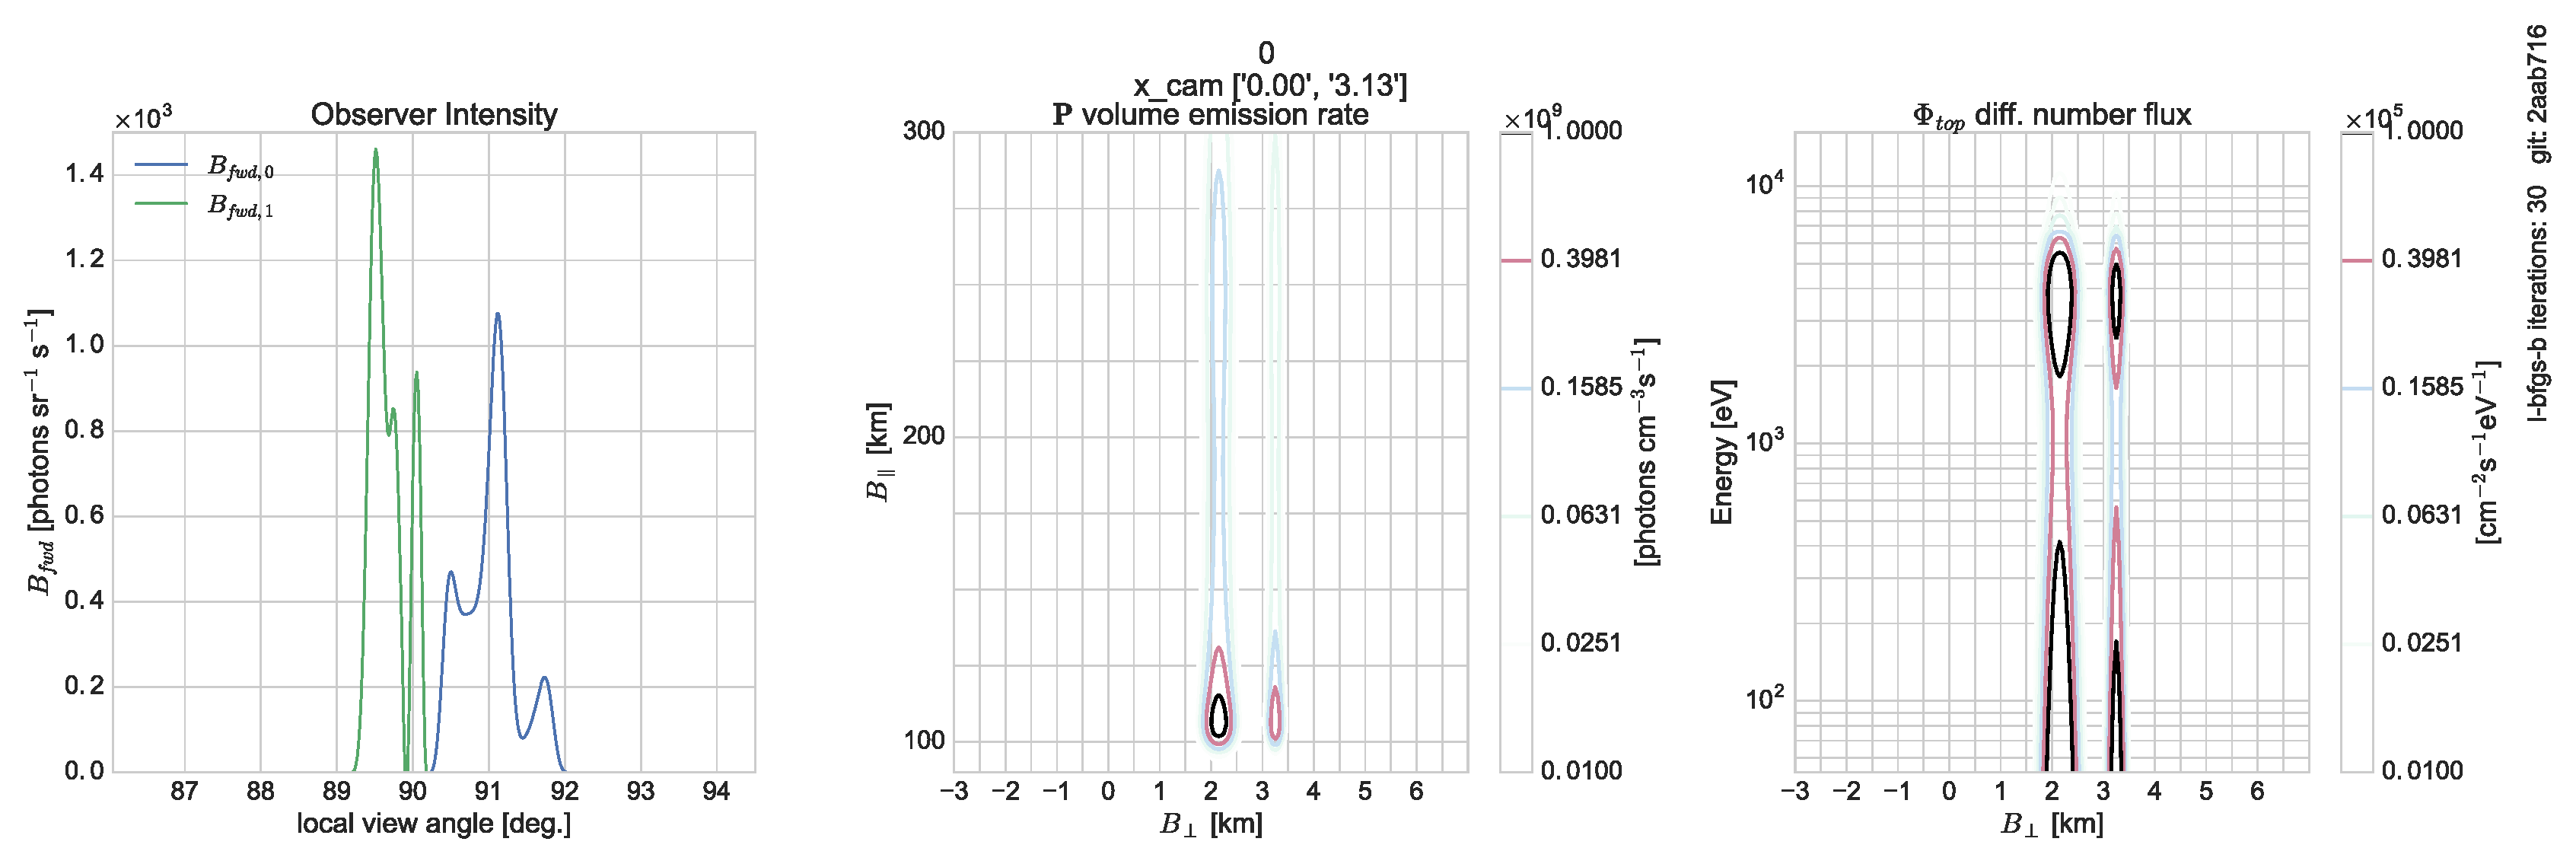
\includegraphics[width=0.9\columnwidth]{gfx/fwd0}
    \caption{Forward model of aurora for HiST two-camera deployment at PFRR. Splitting arc is simulated. 
    	Panel (a) shows ground-observed optical intensity after filtering and wavelength-dependent atmospheric attenuation. 
    	(b) shows the auroral optical volume emission rate vs. $B_\perp$. 
    	(c) shows the unobservable primary electron differential number flux at the ``top'' of the ionosphere, this is the quantity the HiST system estimates with high spatiotemporal resolution.}\label{fig:histfwd}
\end{sidewaysfigure}
\begin{sidewaysfigure}\centering
    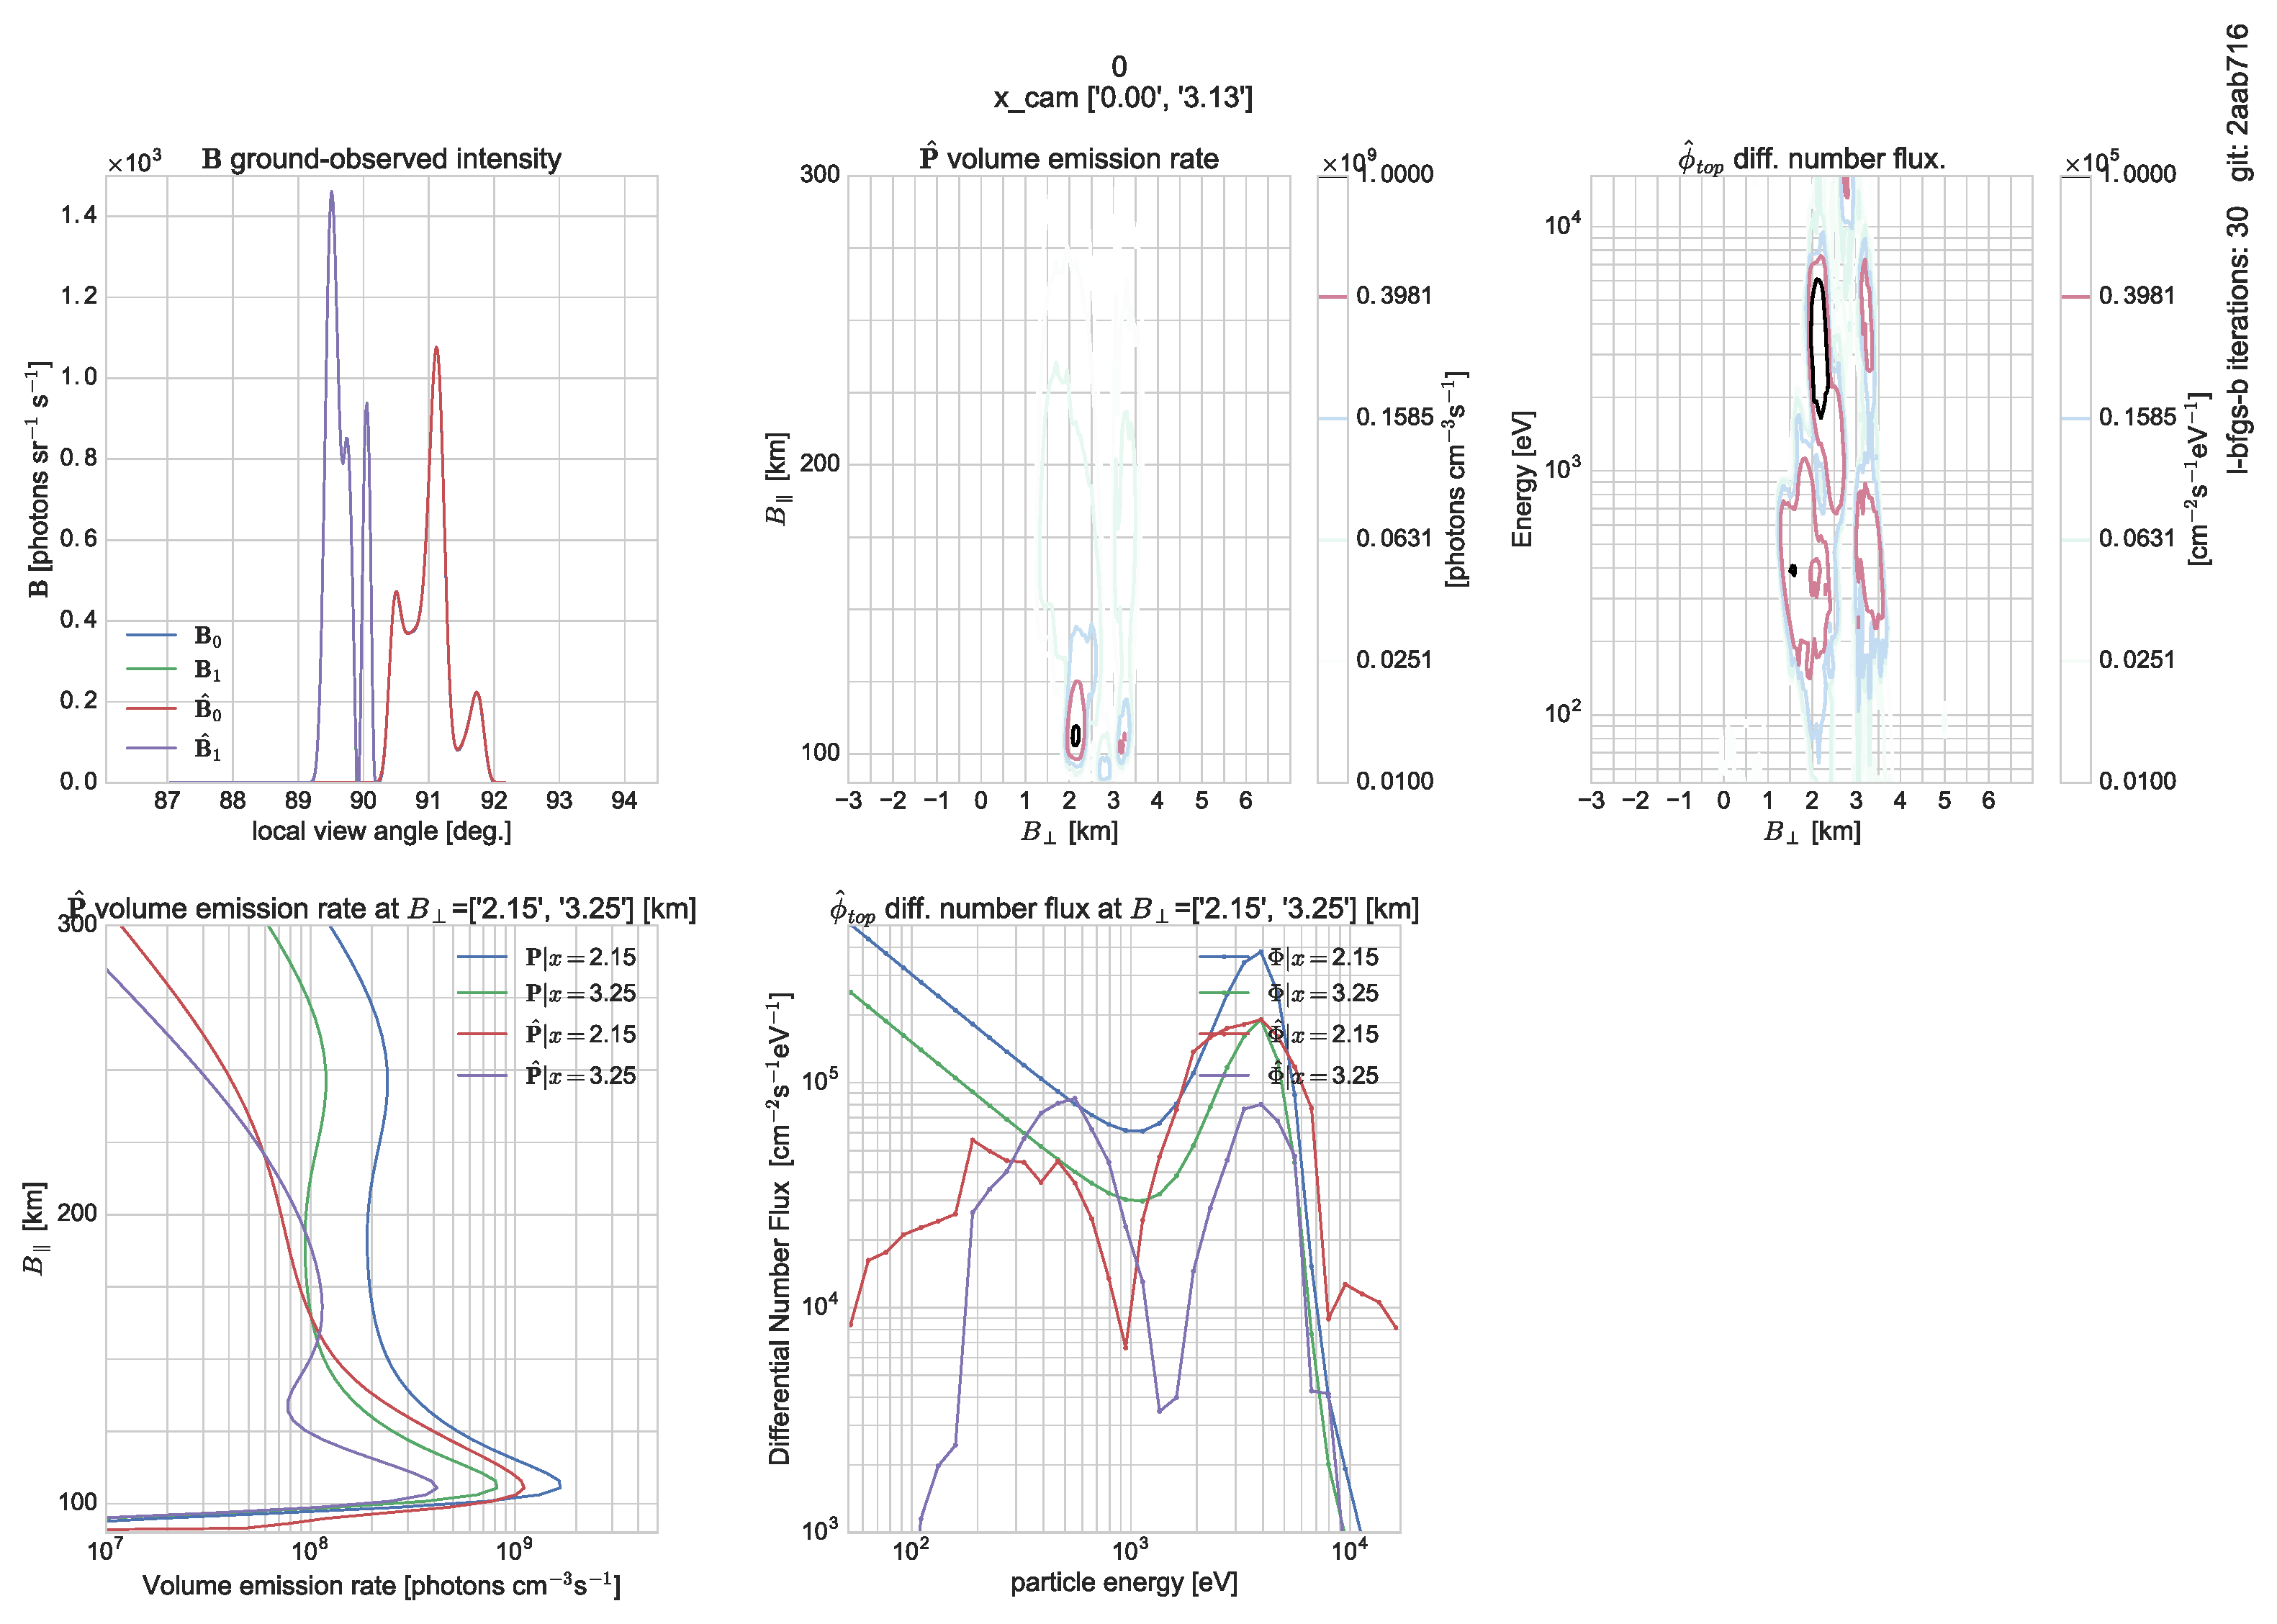
\includegraphics[width=0.75\columnwidth]{gfx/est0}
    \caption{Data inversion for forward modeled HiST two-camera deployment at PFRR. Splitting arc is simulated as in Figure~\ref{fig:histfwd} and precipitation estimated. Panel (a) shows ground-observed and estimated optical intensity after filtering and wavelength-dependent atmospheric attenuation. (b) shows the estimated auroral optical volume emission rate vs. $B_\perp$. (c) shows the estimated primary electron differential number flux at the ``top'' of the ionosphere. (d) shows a 1-D vertical cut of volume emission rate for the two arcs, forward model and estimated. (e) shows a 1-D cut in $B_\perp$ for each arc, forward model and estimated differential number flux.}\label{fig:histest}
\end{sidewaysfigure}

\subsection{Flaming auroral arcs}\label{sec:fusflame}
Flaming aurora manifests as rapidly increasing peak brightness altitude.
The effect can have an appearance like the rapidly rising flames of a campfire, leading to the name for this auroral morphology.
The driving factor behind flaming aurora is dispersive Alfvén waves.
The high energy precipitating particles arrive first in the auroral altitudes of the ionosphere, followed $\sim \unit[100]{ms}$ later by the lower energy particles.

An example flaming auroral arc occurred at PFISR on March 1, 2011 near 10:06 UTC.
Figure~\ref{fig:20110301a}(a) shows pre-Alfvénic arc configuration.
F-region irregularities starting below \unit[300]{km} and rising up to \unit[600]{km} within two seconds are observed in Figure~\ref{fig:20110301a}(b) ISR power with the arrival of high-energy dispersive Alfvénic particles.
\unit[400]{ms} later in Figure~\ref{fig:20110301a}(c), the low-energy Alfvénic flux dominates as the apparent peak altitude of prompt emissions rises rapidly.
Figure~\ref{fig:20110301b}(a) shows the ion-line during the NEIAL altitude climb, with (g) after the NEIAL rose to a more steady altitude.
A few seconds later in Figure~\ref{fig:20110301a}(d), the Alfvénic particle packet has vanished.
Figure~\ref{fig:20110301b}(c) shows the ion-line spectrum without NEIALs present.
Observe that two more NEIAL events occurred before and after the video, but due to the human-initiated record cycle, they were not recorded with video.
\begin{sidewaysfigure}\centering
    % Video
    \includegraphics[width=0.19\columnwidth,trim=30 0 200 0,clip]{gfx/2011-03-01/2040}
    \includegraphics[width=0.261\columnwidth,trim=30 0 60 0,clip]{gfx/2011-03-01/6440}
    \includegraphics[width=0.261\columnwidth,trim=30 0 60 0,clip]{gfx/2011-03-01/6840}
    \includegraphics[width=0.261\columnwidth,trim=30 0 60 0,clip]{gfx/2011-03-01/10440}
    % Power
    \includegraphics[width=\columnwidth,trim=0 50 0 0]{gfx/2011-03-01/power_longpulse2011-03-0110-06-00}\\
    {\large(e)}
    \vspace{0.1cm}

    \caption{Flaming auroral arc sequence at PFISR on March 1, 2011, 10:06 UTC.
        (a) shows pre-Alfvénic arc configuration.
        (b) F-region irregularities are observed in the ISR power (e) with the arrival of high-energy DAW accelerated electron.
        (c) \unit[400]{ms} later, the low-energy Alfvénic flux dominates as the apparent peak altitude of prompt emissions rises rapidly.
        (d) the Alfvénic particle packet has vanished.
        (e) ISR backscatter showing three NEIAL events in series--video only available for middle event.}
    \label{fig:20110301a}
\end{sidewaysfigure}

\begin{figure}\centering
    % Psd
    \includegraphics[width=0.5\columnwidth,trim=0 50 0 0]{gfx/2011-03-01/acfslice_longpulse2011-03-0110-06-11}

    \vspace{-1cm}(a)
    \vspace{1cm}

    \includegraphics[width=0.5\columnwidth,trim=0 50 0 0]{gfx/2011-03-01/acfslice_longpulse2011-03-0110-06-17}

    \vspace{-1cm}(b)
    \vspace{1cm}

    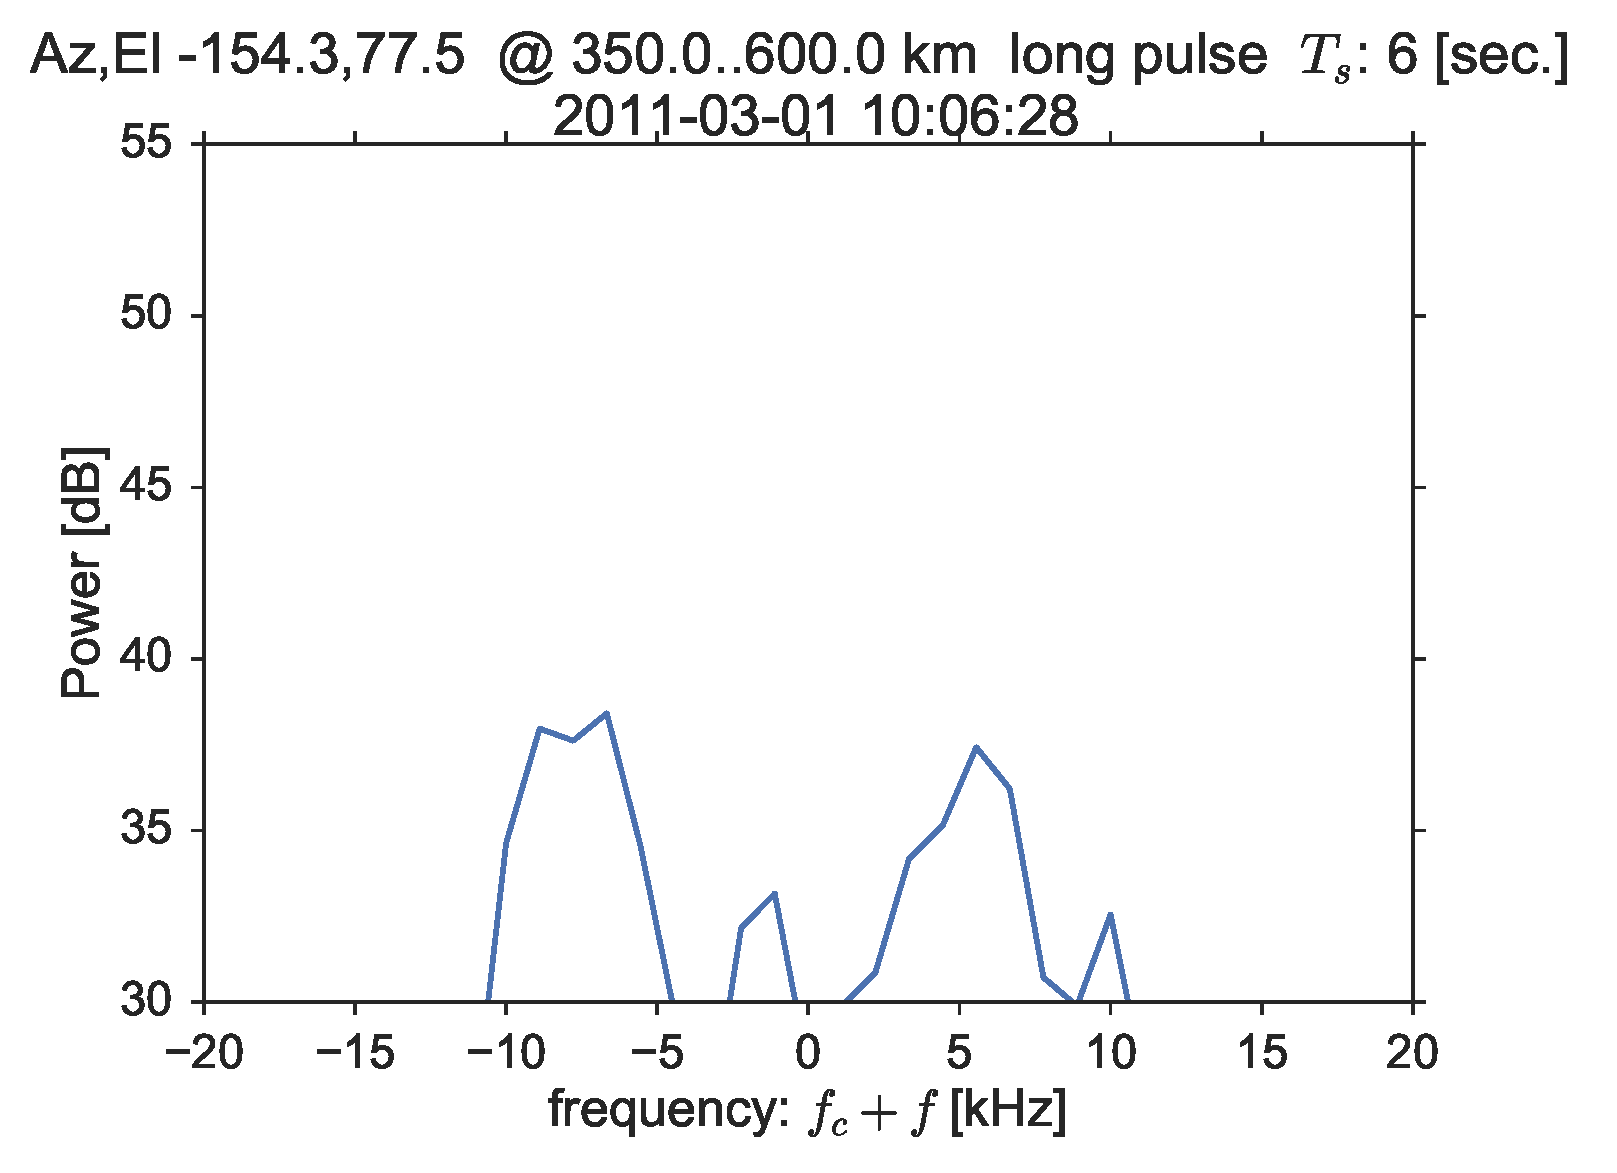
\includegraphics[width=0.5\columnwidth,trim=0 50 0 0]{gfx/2011-03-01/acfslice_longpulse2011-03-0110-06-28}

    \vspace{-1cm}(c)
    \vspace{1cm}

	%(a)\hspace{0.275\columnwidth}(b)\hspace{0.275\columnwidth}(c)

	\caption{Flaming auroral arc sequence at PFISR on March 1, 2011.
    (a,b) show enhanced negative frequency shift ion-acoustic line.
    (c) shows normal ion-acoustic line.}
    \label{fig:20110301b}
\end{figure}

Only a single high-speed sCMOS was running at 30 frames/s, in burst recording mode of several seconds each manual record start.
Context for the event is provided by PF-DMSP in Figure~\ref{fig:msp20110301} and GIMA in Figure~\ref{fig:mag20110301}.
\begin{figure}\centering
    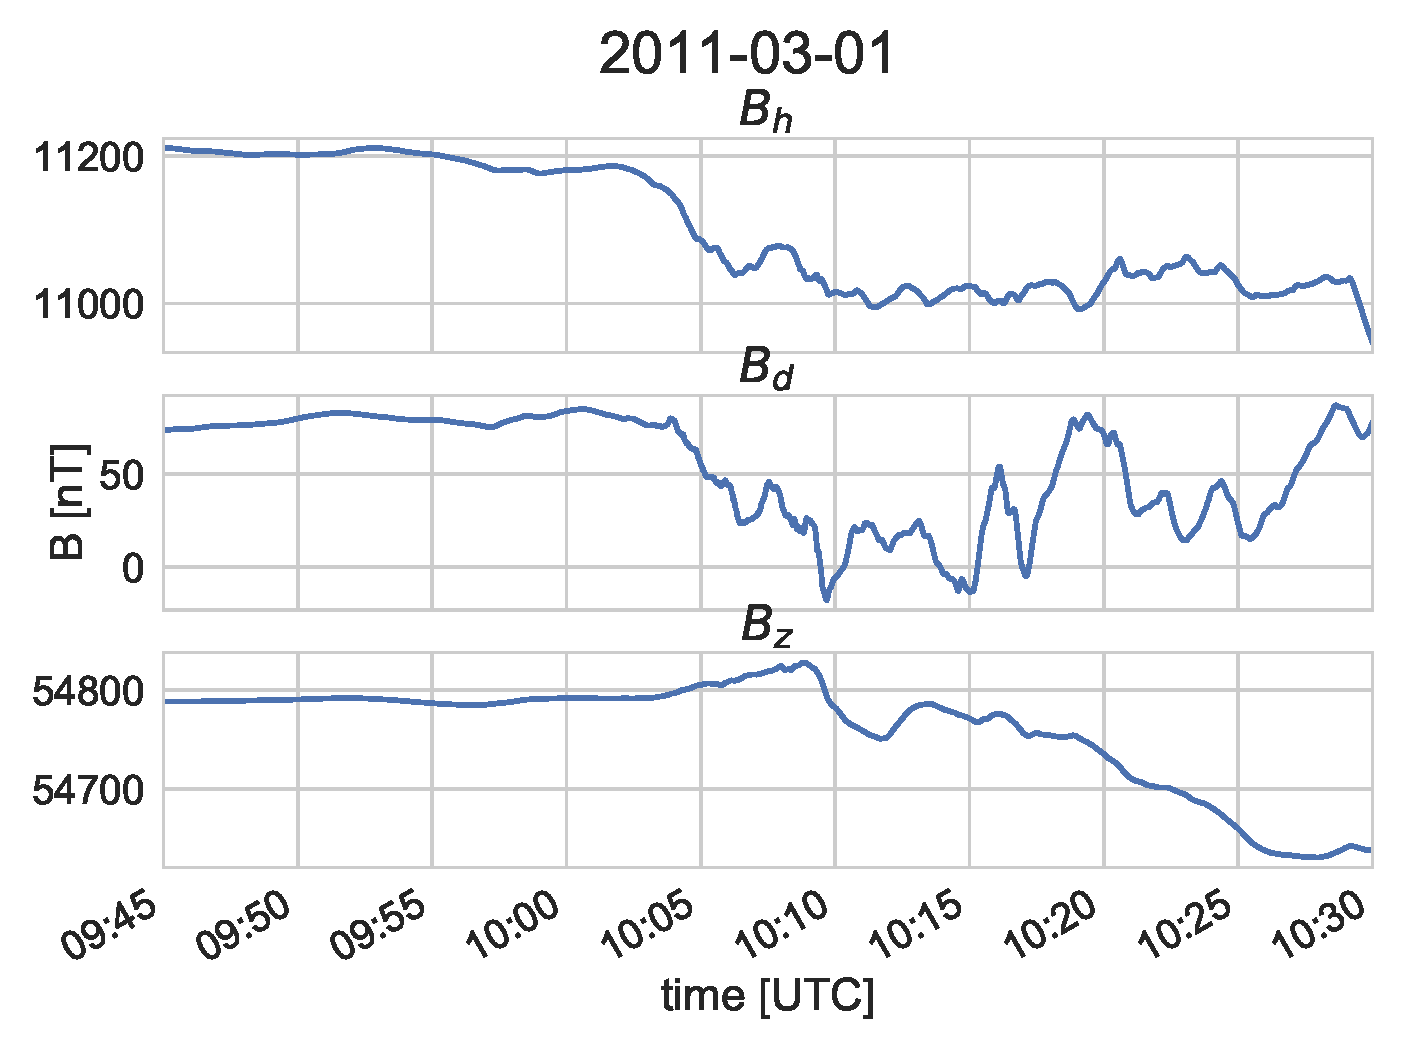
\includegraphics[width=\columnwidth]{gfx/2011-03-01/mag}
    \caption{Quiet conditions before the flaming auroral event are perturbed during the 2011-03-01 substorm.}
    \label{fig:mag20110301}
\end{figure}
The PF-DMSP spectrum of Figure~\ref{fig:msp20110301} had $I_{555.7}$ and $I_{427.8}$ available.
\begin{figure}\centering
    \includegraphics[width=\columnwidth]{gfx/2011-03-01/msp_ratio}
    \caption{PF-DMSP (a) $I_{555.7}$ and (b) $I_{427.8}$ with ratio (c) $I_{555.7} / I_{427.8}$. Around 10:06 and 10:11 UTC  intensifications near magnetic zenith indicates large increase in characteristic energy.}
    \label{fig:msp20110301}
\end{figure}
According to \citet{rees1974}, the magnetic zenith energies are on the order of \unit[5..10]{keV} during this event.
The PF-DMSP data is highly smeared in time across this event.
\citet{dahlgren2013} provided estimates using assumptions on the starting altitude of the flaming feature in a single-camera data inversion.
HiST was designed to study this type of event, with long-term automated recording so that events are not missed and the precipitation energy dynamics can be examined in more quantitative detail.

\FloatBarrier
\subsection{Kinked auroral arc}\label{sec:kink}
Auroral arcs with folds or kinks originate with magnetospheric configurations that are non-dispersive in nature.
Such disturbances also drive auroral vortices and vortex streets.
A striking example of a kinked auroral arc is shown in Figure~\ref{fig:20130414T0826}.
\begin{sidewaysfigure}\centering
    \noindent\includegraphics[width=\columnwidth,trim=15 697 25 0,clip]{gfx/2013-04-14T0826/2013-04-14T0826}

    \hspace{1.1cm}(a) 08:26:07.400 UT 
    \hspace{1.25cm}(b) 08:26:08.000 UT
    \hspace{1.1cm}(c) 08:26:08.100 UT
    \hspace{1.1cm}(d) 08:26:12.000 UT
    
    \caption{Narrow kinking and translating arcs at PFISR, ca. 08:26:10 UTC on April 14, 2013. 
          No coherent echoes detected in ion line, plasma line, or power spectral density.}
    %Two satellites cross through the field of view nearly orthogonally at 08:24:18 UTC.
    \label{fig:20130414T0826}
\end{sidewaysfigure}
A substorm is indicated as the initiator of the perturbation based on the southward turning IMF reflected in sharp negative excursion at 08:25 UTC as shown in Figure~\ref{fig:mag0826}.
\begin{figure}\centering
    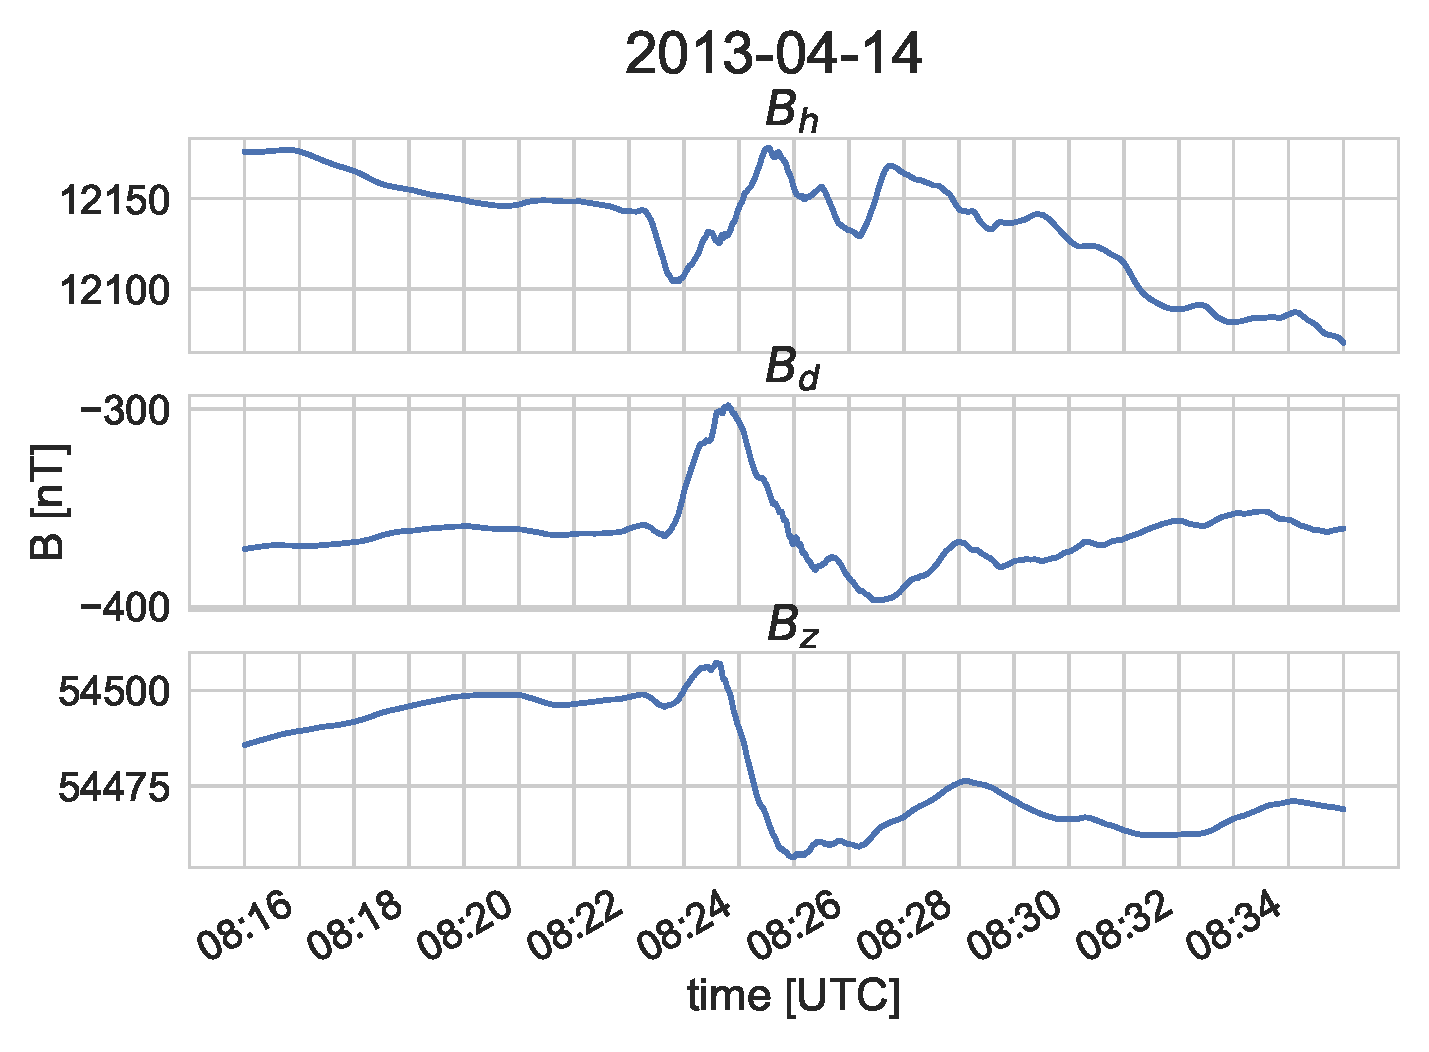
\includegraphics[width=\columnwidth]{gfx/2013-04-14T0826/mag}
    \caption{GIMA PFRR data showing geomagnetic field reversal near 08:25 UTC.}
    \label{fig:mag0826}
\end{figure}
A likely driver for this arc structure is an inverted-V acceleration region.
%As observed with HiST the auroral spectrum including the lines of Figure~\ref{fig:msp0826} is passed through the HiST BG3 filter, yielding $I_{557.7} \sim 0.01 \times I_{427.8}$.
The $I_{427.8}$ intensity suggests monoenergetic several keV electron beam configuration.
\begin{figure}
    \includegraphics[width=\columnwidth]{gfx/2013-04-14T0826/msp_spectra}
    \caption{PF-DMSP spectrum showing strong $I_{427.8}$, suggesting monoenergetic beam of several keV driving kinked arc near 08:26 UTC.}\label{fig:msp0826}
\end{figure}
Monoenergetic inverted-V accelerated electron differential number flux in the several keV range is the most likely candidate for generating this kinked aurora.
\section{Discussion and Conclusions}\label{sec:disc}
In-situ measurements obtained from sounding rockets have long established that intense Langmuir waves with amplitudes approaching \unit[1.2]{V/m} are common features of the auroral ionosphere. 
Langmuir waves are observed propagating nearly parallel to $B$ and occur in bursts with durations of hundreds of milliseconds \citep{mcfadden1986,boehm1984,ergun1999a,ergun1999b}.
Freja observations confirm that Langmuir waves are the strongest electrostatic waves at altitudes $\sim \unit[1500]{km}$ \citep{stasiewicz1996}.
Such Langmuir waves have been suggested to play an important role in the auroral ionosphere energy flow chain, facilitating energy transfer from AW to the bulk plasma \citep{stasiewicz1996}.

Although observation of intense Langmuir waves in the ionosphere is not a new finding, the significance of ISR detected Langmuir turbulence lies in the specific wavenumber at which ISR-detectable wave activities are enhanced. 
The detection of Langmuir waves at relatively high wave numbers: $k \sim \unit[19]{m^{-1}}$ for PFISR and $k \sim \unit[39]{m^{-1}}$  for EISCAT puts constraints on the dynamics of interactions and/or on the characteristics of the underlying energy source for the enhanced waves \citep{akbari2014}.
Furthermore, there seems to be discrepancies between ISR and in-situ observations:
\begin{enumerate}
    \item \textit{in situ} measurements suggest that Langmuir turbulence should be commonly observed at altitudes above 600~km, whereas the ISR echoes are seen consistently at the F-region peak around 250-300 km.
    \item ISR measurements suggest that the intense Langmuir waves generate a well-developed turbulence which leads to caviton formation and collapse, whereas signatures of caviton formation have been completely missing in the \textit{in situ} measurement literature, with the exception of the inconclusive results of \citet{boehm1984}.
    \item \textit{In situ} measurements have shown that the enhanced Langmuir waves at higher altitudes are rather monochromatic \citep{ergun1999a,ergun1999b}. 
\end{enumerate}

A portion of the apparent inconsistencies between ISR and \textit{in situ} measurements may naturally arise from the different dynamics of beam-plasma interactions expected at different altitudes (i.e. \unit[250..300]{km} versus $>\unit[600]{km}$).
However, one should be cautious about drawing a definite conclusion that the processes underlying the radar echoes are just a low-altitude extension of the beam-plasma interactions long known from \textit{in situ} measurements.

An aspect of the ISR observations that bears discussion is the source of free energy underlying the detected turbulence.
In natural plasmas a common mechanism for intensification of Langmuir waves is the bump-on-tail instability (or inverse Landau damping) which operates upon the existence of a bump (positive slope) on the reduced (one-dimensional) electron velocity distribution function. 
This bump often represents the existence of an additional population of electrons on top of the bulk electrons. 
This population could be locally produced via acceleration or energization of a portion of the local electrons, or it could consist of electrons traveling to the observer in the form of electron beams. 
In the lower ionosphere and in the absence of any known local acceleration mechanism, a bump on the distribution function may directly arise from:
\begin{enumerate}
    \item the auroral magnetospheric-origin electron beams that are accelerated at high altitudes and propagate to the lower ionosphere (with energies of hundreds of eV to a few keV or more)
    \item the secondary electron population (with energies of a few eV to $\sim \unit[100]{eV}$) that emerges as a result of collisional interactions of the primary auroral electrons with the Earth's neutral atmosphere.
\end{enumerate}
In the former case, it is crucial to make a distinction between the electron beams accelerated by inertial AW and the inverted-V electron beams accelerated by quasi-static parallel electric fields. 

Detection of Langmuir waves in the ISR plasma-line channels enables the determination of the phase velocity $v_\varphi=\omega / k$ of the Langmuir waves and consequently the energy of the electrons directly exchanging energy with the waves. 
For PFISR observations, this energy is $\sim \unit[5]{eV}$, which falls in the energy range of secondary electrons. 
This may suggest that the secondary electrons provide the energy for the turbulence. 
Secondary electrons are known to be responsible for intensification of Langmuir waves in the E-region of the auroral ionosphere \citep{nilsson1996}. 
Langmuir wave intensification in such cases is associated with the presence of a bump, itself associated with the absorption cross-section of $N_2$, in the three-dimensional distribution function which results in reduction of Landau damping and increase in the Čerenkov emission rate. 
However, numerical modelings \citep{nilsson1996} have show that this bump appears over a broad range of pitch angles and is nearly isotropic at lower altitudes of the E-region and do not produce a bump in the reduced (one-dimensional) distribution function. 
As such, the plasma remains stable and the intensification of Langmuir waves is limited. 
At higher altitudes, the secondary electron spectra further deviate from isotropic; however, the pump becomes less pronounced due to the change in the neutral gas composition.

In summary, although secondary electrons have been suggested to cause plasma instabilities involving wave modes propagating nearly perpendicular to the magnetic field lines \citep{basu1982,jasperse2013}, are generally considered stable with respect to Langmuir waves. 
An additional evidence against the secondary electrons as the energy source for the F region Langmuir turbulence echoes, exists in the ISR data; where no correlation between the E region ionization (which is proportional to the secondary electron production rate) and the Langmuir turbulence echoes is found \citep{akbari2013}. 
It is also worth mentioning that the presence of secondary electrons with power law-like distributions, not only does not lead to instability, but instead significantly weakens the turbulence via introducing enhanced Landau damping to Langmuir waves \citep{newman1994linear,newman1994nonlinear,akbari2015}. 

The problem regarding the primary energetic auroral electrons as the source of energy for the turbulence underlying the radar echoes is that the Langmuir waves that are directly in energy exchange with such energetic electrons have wave numbers far below the detecting wave numbers of the existing incoherent scatter radars and, as such are undetectable.
Assuming that the parametric decay of Langmuir waves is the main product of the beam-plasma interactions at the observation altitudes, the energy transfers to yet smaller wave numbers, via a cascade of PDIs, and further away from the radar wavenumber. 
However, it has been shown that a well developed Langmuir turbulence does transfer a small fraction of the input energy to higher wave numbers via processes such as the caviton collapse or three-wave coalescence-like interactions \citep{akbari2014,akbari2015}, and that these could be the origin of the observed ISR echoes. 
Therefore, the possibility that the primary auroral electron beams are the direct source of the turbulence may not be ruled out.

It is necessary to make a distinction between the two types of electron beams that are commonly observed in the auroral ionosphere, i.e. the inverted-V electron beams and the field-aligned electron bursts. 
The inverted-V electron beams are produced by acceleration of warm plasma sheet electrons via quasi-static parallel electric fields at the earth acceleration region. 
It is possible for the inverted V electron beams to produce a positive slope in the one-dimensional distribution function at high altitudes close to the acceleration region. 
However, in short time scales and before the beams have the chance to travel long distances, the self-generated plasma waves quickly plateau the positive slope via  quasi-linear diffusion \citep{sanbonmatsu2001}, rapidly stabilizing the distribution. 
In addition to the quasilinear diffusion, while traveling from the acceleration region toward the ionosphere, the inverted-V electron beams become subject to adiabatic evolution under the converging magnetic field limes. 
As a result of the magnetic mirror force, the field-aligned beam diffuses toward oblique and perpendicular directions \citep{maggs1981}, which although leading to intensification of oblique propagating wave modes such as the upper-hybrid and whistler modes \citep{maggs1978,kaufmann1980,maggs1981}, further stabilize the distribution against Langmuir waves. 

Sounding rocket measurements of the three-dimensional electron velocity distributions at F-region altitudes, have consistently shown that the inverted-V electron beams often have a broad, nearly isotropic plateau that despite having a positive slope in the three-dimensional distribution function, does not produce a positive slope in the reduced (one-dimensional) distribution function in near parallel directions \citep{kaufmann1978,kaufmann1980,mcfadden1986}.
Such distributions are, therefore, stable against Langmuir turbulence. 
This general rule, however, may not be correct universally. 
From the experimental point of view, given the low temporal resolution of the electron velocity distribution function measurements, the existence of transient positive slopes in time scales shorter than the measurement resolutions may not be completely ruled out. 
Also from the theoretical point of view, a number of linear (wave refraction) \citep{maggs1978} and nonlinear (parametric type instabilities) \citep{papad1974} mechanisms have been suggested to be able to limit the growth of the beam-generated electrostatic waves and, consequently, limit the quasi-linear flattening of the beam, ultimately enabling the beam to maintain its unstable features while traveling down to the F-region altitudes. 
While such considerations can not be completely ruled out, a final evidence against the inverted-V electron beams as the source of turbulence underlying the ISR echoes, lies in the ISR data itself, where no correlation between the E-region ionization enhancements (the signature of energetic electron precipitation) and the turbulence echoes are found.

In contrast to inverted-V electron beams, field-aligned electron bursts produced by acceleration of cold ionospheric electrons via parallel electric field of inertial Alfvén waves \citep{kletzing2001,semeter2008} have characteristics that make them suitable candidates as the energy source for Langmuir wave enhancement at various altitudes. 
An important characteristic of the field-aligned bursts is their velocity dispersion, where the characteristic energy of the beam decreases from a few keV to $\sim\unit[100]{eV}$ over a period of $\sim \unit[100]{ms}$ (for a description of field-aligned bursts see \citet{mcfadden1987}). 
This dispersive behavior plays a major role in maintaining the beam distribution by continuously reproducing the positive slope of the distribution function, once flattened by the quasilinear diffusion, enabling the beam to remain unstable as it travels deep into the ionosphere \citep{ergun1993,sanbonmatsu2001}. 
This same behavior has been studied in the context of Langmuir wave enhancement in the solar wind and the type III radio bursts \citep{muschietti1990}. 

\textit{In situ} measurements obtained with sounding rockets have long established the connection between intense Langmuir waves in the auroral ionosphere and dispersive field-aligned electron bursts \citep{ergun1999a,stasiewicz1996}. 
Intense Langmuir waves observed \textit{in situ} are seen to undergo various non-linear interactions \citep{boehm1987,gough1990,ergun1999b}.
The association of:
\begin{enumerate}
    \item intense Langmuir waves with ISR Langmuir turbulence echoes
    \item dispersive Alfvénic accelerated electron beams with the source of energy underlying the echoes
\end{enumerate}  
are not obvious conclusions due to a number of discrepancies between the in-situ and ISR observations. 
Making such a connection, therefore, requires additional evidence as provided in this chapter from the joint HiST-PFISR observations.
Using the events presented in this paper and supplemental material, Table \ref{tab:events} collects the evidence for Alfvénic arcs corresponding to NEIALs.
\begin{sidewaystable}\centering
    \caption{Morphologies of events detailed in the paper and supplemental material. SLT=Strong Langmuir Turbulence}
    \label{tab:events}
    \begin{tabular}{lllll}
        \toprule
        Event Time [UT] & Aurora Morphology & ISR Morphology & Plasma Morphology & Figure \\
        \midrule
%        2007-03-18 & translating frozen-in & TODO & TODO & \\ % waiting SRI data
        2007-03-23 & splitting, flaming & 30 dB SNR ion line & SLT & \\
        2011-03-01 10:06 & flaming & $\Uparrow30$ dB ion line & Streaming upflow & \ref{fig:20110301a}, \ref{fig:20110301b} \\
%        2011-03-02 & & &  & \\
%        2012-11-07 & & & & \\
%        2013-04-01 & & & & \\
%        2013-04-04 & & & & \\
%        2013-04-07 & & & & \\
%        2013-04-11 & & & & \\
        2013-04-14 08:26 & Kinked, vortical & quiet & Thermal & \ref{fig:20130414T0826} \\
        2013-04-14 08:54 & Splitting/shedding & $\Uparrow30$ dB ion \& plasma lines & SLT & \ref{fig:20130414T0854a}, \ref{fig:20130414T0854b} \\
%        2013-04-14 09:27 & dark patches and flickering & quiet & Thermal & \ref{fig:20130414T0927}\\
%        2013-04-20 & & & & \\
%        2013-04-23 & & & & \\
%        2013-04-26 & & & & \\
%        2013-05-01 & & & & \\
        \bottomrule
    \end{tabular}
\end{sidewaystable}
The initial observations of the limited set of aurora and ISR turbulence presented suggests the following correspondence:
\begin{enumerate}
    \item inverted-V $\impliedby$ kinked aurora (Figure~\ref{fig:cartoonmorph}(a))
    \item strong Langmuir turbulence (F region) $\leftrightarrows$ splitting aurora (Figure~\ref{fig:cartoonmorph}(b))
    \item streaming upflow ($> 600$~km altitude)  $\leftrightarrows$ flaming aurora (Figure~\ref{fig:cartoonmorph}(c))
    
\end{enumerate}

\subsection{Future experimental configuration}\label{sec:future}
Using the BG3-filtered broadband prompt emission lines and bands captured by HiST cameras \citep{hirsch2016}, estimates of primary electron differential number flux with time scales fast enough to capture DAW behavior can be imaged and quantified.
Since the imaging chip provides a weighted sum of all emissions passing through the BG3 filter, spectral information is lost.
Existing spectrometers and hyper-spectral imagers \citep{goenka2016} typically have frame rates on the order of seconds to minutes.
The latest generation of EMCCD technology has $1024 \times 1024$ pixels at \unit[25]{fps}, nearly as fast as HiST imagers. 
A spectrograph is being tested for field deployment next year, colocated with HiST and with a similar FOV to resolve specific auroral emission lines. 
This additional data will help quantify the chemistry responsible for a discrete arc viewed by HiST, yielding further insights into the kinetics responsible for NEIALs.